% !TEX program = pdflatex
\documentclass[aspectratio=169, 10pt]{beamer}
\usepackage[utf8]{inputenc}
\usepackage[T1]{fontenc}
\usepackage{graphicx}
\usepackage{booktabs}
\usepackage{amsmath}
\usepackage{amssymb}
\usepackage{tikz}
\usepackage{xcolor}

\usetikzlibrary{arrows.meta, positioning, calc, shapes.geometric}

\usetheme{Cuerna}
\usecolortheme{bluesimplex}

\graphicspath{{../results/}}

% --- Custom colors ---
\definecolor{neuralblue}{HTML}{3469CC}
\definecolor{classicalred}{HTML}{BD2026}
\definecolor{findinggreen}{HTML}{2E8B57}
\definecolor{darkgray}{HTML}{282d33}

% --- Slide numbers ---
\setbeamertemplate{footline}{%
  \hfill{\scriptsize \insertframenumber{}/\inserttotalframenumber}\hspace*{8pt}\vspace{6pt}%
}

% --- Add IIITD logo to all slides ---
\logo{
\includegraphics[height=0.8cm]{image.png}}
\titlegraphic{
\includegraphics[width=2.5cm]{image.png}}

% --- Decrease global margins mildly to maximize space ---
\setbeamersize{text margin left=0.6cm,text margin right=0.6cm}

% --- Metadata ---
\title{Neural Differential Cryptanalysis}
\subtitle{A Systematic Study on SPECK32/64}
\author{Angadjeet Singh --- 2022071}
\institute{Applied Cryptography \\ Department of CSE, IIIT Delhi}
\date{April 2026}

\begin{document}

% ==============================================================================
% SLIDE 1: Title
% ==============================================================================
\begin{frame}[plain]
  \titlepage
\end{frame}

% ==============================================================================
% SLIDE 2: Outline
% ==============================================================================
\begin{frame}{Outline}
\small
\begin{enumerate}
  \setlength{\itemsep}{0.2cm}
  \item \textbf{Motivation} --- Why neural cryptanalysis?
  \item \textbf{Background} --- Differential cryptanalysis \& SPECK32/64
  \item \textbf{Research Questions \& Experimental Setup}
  \item \textbf{Core Results}
  \begin{itemize}
    \item Baseline $\cdot$ Representation $\cdot$ Saliency $\cdot$ Robustness $\cdot$ Markov
  \end{itemize}
  \item \textbf{Extended Analysis}
  \begin{itemize}
    \item Neural vs.\ classical $\cdot$ Gen/Latent $\cdot$ Architecture $\cdot$ Efficiency
  \end{itemize}
  \item \textbf{Key Findings \& Future Work}
\end{enumerate}
\end{frame}

% ==============================================================================
% SLIDE 3: Hook / Motivation
% ==============================================================================
\begin{frame}{Can Neural Networks Break Ciphers?}
\small
\begin{columns}[T]
\begin{column}{0.55\textwidth}
\textbf{Classical differential cryptanalysis:}
\begin{itemize}
  \item Manual search over propagation tables
  \item Deep domain expertise per cipher
  \item Exponential search space at higher rounds
\end{itemize}

\textbf{Gohr (CRYPTO 2019):}
\begin{itemize}
  \item Neural network as a \emph{distinguisher}
  \item 92.4\% accuracy on 5-round SPECK32/64
  \item Outperformed classical tests at 7--8 rounds
\end{itemize}

\textbf{Open question:}\\
\emph{Where} does the signal reside, and \emph{how} do networks extract it?
\end{column}
\begin{column}{0.40\textwidth}
\centering
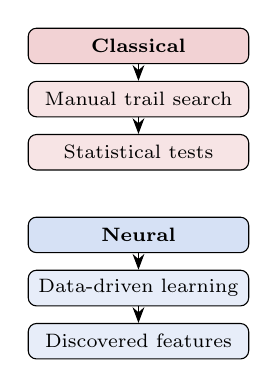
\begin{tikzpicture}[scale=0.75, every node/.style={font=\scriptsize},
  box/.style={draw, rounded corners=3pt, minimum width=2.8cm, minimum height=0.45cm, align=center}]
  \node[box, fill=classicalred!20, font=\scriptsize\bfseries] (trad) at (0,3.2) {Classical};
  \node[box, fill=classicalred!12] (manual) at (0,2.3) {Manual trail search};
  \node[box, fill=classicalred!12] (stat) at (0,1.4) {Statistical tests};
  \draw[-{Stealth[length=2mm]}] (trad) -- (manual);
  \draw[-{Stealth[length=2mm]}] (manual) -- (stat);

  \node[box, fill=neuralblue!20, font=\scriptsize\bfseries] (neural) at (0,0) {Neural};
  \node[box, fill=neuralblue!12] (data) at (0,-0.9) {Data-driven learning};
  \node[box, fill=neuralblue!12] (learn) at (0,-1.8) {Discovered features};
  \draw[-{Stealth[length=2mm]}] (neural) -- (data);
  \draw[-{Stealth[length=2mm]}] (data) -- (learn);
\end{tikzpicture}
\end{column}
\end{columns}
\end{frame}

% ==============================================================================
% SLIDE 4: Background
% ==============================================================================
\begin{frame}{Differential Cryptanalysis \& SPECK32/64}
\small
\begin{columns}[T]
\begin{column}{0.50\textwidth}
\textbf{Core idea:} trace input-difference propagation.
\[
\Delta P = P \oplus P' \;\longrightarrow\; \Delta C = E_k(P) \oplus E_k(P')
\]
\textbf{Differential probability:}
\[
\text{DP} = \frac{|\{x : F(x) \oplus F(x \oplus \Delta P) = \Delta C\}|}{2^n}
\]
\textbf{Markov assumption:} multi-round probability = product of single-round probabilities.

\textbf{SPECK32/64:}\\
ARX cipher. 32-bit block, 64-bit key, 22 rounds.\\
$\Delta P = \texttt{0x0040\_0000}$. Rounds 3--9.
\end{column}
\begin{column}{0.46\textwidth}
\centering
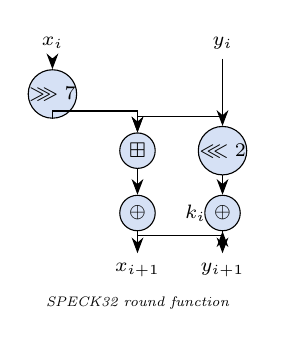
\begin{tikzpicture}[scale=0.72, every node/.style={font=\scriptsize},
  op/.style={draw, circle, fill=neuralblue!20, minimum size=0.45cm, inner sep=0pt, font=\scriptsize\bfseries}]
  \node (x) at (0,4.5) {$x_{i}$};
  \node (y) at (3.0,4.5) {$y_{i}$};

  \node[op] (rr) at (0,3.6) {$\ggg 7$};
  \draw[-{Stealth[length=2mm]}] (x) -- (rr);

  \node[op] (add) at (1.5,2.6) {$\boxplus$};
  \draw[-{Stealth[length=2mm]}] (rr) -- ++(0,-0.3) -| (add);
  \draw[-{Stealth[length=2mm]}] (y) -- ++(0,-1.3) -| (add);

  \node[op] (xk) at (1.5,1.5) {$\oplus$};
  \node[right=0.25cm] at (xk.east) {$k_i$};
  \draw[-{Stealth[length=2mm]}] (add) -- (xk);

  \node[op] (rl) at (3.0,2.6) {$\lll 2$};
  \draw[-{Stealth[length=2mm]}] (y) -- (rl);

  \node[op] (xf) at (3.0,1.5) {$\oplus$};
  \draw[-{Stealth[length=2mm]}] (rl) -- (xf);
  \draw[-{Stealth[length=2mm]}] (xk) -- ++(0,-0.4) -| (xf);

  \node (xo) at (1.5,0.5) {$x_{i+1}$};
  \node (yo) at (3.0,0.5) {$y_{i+1}$};
  \draw[-{Stealth[length=2mm]}] (xk) -- (xo);
  \draw[-{Stealth[length=2mm]}] (xf) -- (yo);

  \node[below, font=\tiny\itshape] at (1.5, 0.2) {SPECK32 round function};
\end{tikzpicture}
\end{column}
\end{columns}
\end{frame}

% ==============================================================================
% SLIDE 5: Neural Distinguishers
% ==============================================================================
\begin{frame}{Neural Distinguishers}
\small
\begin{columns}[T]
\begin{column}{0.50\textwidth}
Reframe distinguishing as \textbf{binary classification}:
\[
D_\theta : \{0,1\}^n \times \{0,1\}^n \to [0,1]
\]
\begin{itemize}
  \item $y\!=\!1$: real cipher pair $(C, C')$
  \item $y\!=\!0$: uniformly random pair
  \item Loss: binary cross-entropy
  \item 50\% accuracy $=$ no signal
\end{itemize}

\textbf{Advantage:}
\[
\text{Adv} = |\Pr[D\!=\!1 | y\!=\!1] - \Pr[D\!=\!1 | y\!=\!0]|
\]
Learns non-linear decision boundary from data --- sidesteps sparse-sample DP.
\end{column}
\begin{column}{0.46\textwidth}
\centering
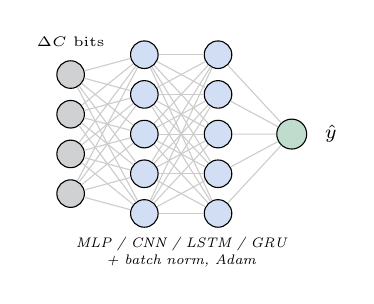
\begin{tikzpicture}[scale=0.72, every node/.style={font=\scriptsize},
  neuron/.style={draw, circle, fill=neuralblue!22, minimum size=0.35cm, inner sep=0pt}]
  \foreach \i in {1,...,4} {
    \node[neuron, fill=darkgray!22] (i\i) at (0, 3.2-\i*0.7) {};
  }
  \node[above=0.05cm, font=\tiny] at (i1.north) {$\Delta C$ bits};
  \foreach \i in {1,...,5} {
    \node[neuron] (h1\i) at (1.3, 3.55-\i*0.7) {};
  }
  \foreach \i in {1,...,5} {
    \node[neuron] (h2\i) at (2.6, 3.55-\i*0.7) {};
  }
  \node[neuron, fill=findinggreen!30, minimum size=0.38cm] (o) at (3.9, 1.45) {};
  \node[right=0.1cm] at (o.east) {$\hat{y}$};
  \foreach \i in {1,...,4} {
    \foreach \j in {1,...,5} {
      \draw[thin, gray!40] (i\i) -- (h1\j);
    }
  }
  \foreach \i in {1,...,5} {
    \foreach \j in {1,...,5} {
      \draw[thin, gray!40] (h1\i) -- (h2\j);
    }
  }
  \foreach \i in {1,...,5} {
    \draw[thin, gray!40] (h2\i) -- (o);
  }
  \node[below, font=\tiny\itshape, text width=3cm, align=center] at (1.95, -0.2) {MLP / CNN / LSTM / GRU\\+ batch norm, Adam};
\end{tikzpicture}
\end{column}
\end{columns}
\end{frame}

% ==============================================================================
% SLIDE 6: Research Questions & Setup
% ==============================================================================
\begin{frame}{Research Questions \& Experimental Setup}
\small
\begin{columns}[T]
\begin{column}{0.48\textwidth}
\textbf{RQ1 --- Representation:}\\
How does input preprocessing affect accuracy?

\textbf{RQ2 --- Markov Assumption:}\\
Does the classical memoryless assumption hold?

\textbf{RQ3 --- Architecture:}\\
Best accuracy-efficiency tradeoff?

\textbf{Setup:}
\begin{itemize}
  \item 15 experiments on SPECK32/64
  \item 7 input representations (R1--R5, R8, R9)
  \item 6 architectures
  \item 10M train / 1M test per config
  \item 5 seeds, bootstrap 95\% CIs
\end{itemize}

{\tiny \textit{pp} = percentage points (absolute gap).}
\end{column}
\begin{column}{0.48\textwidth}
\centering
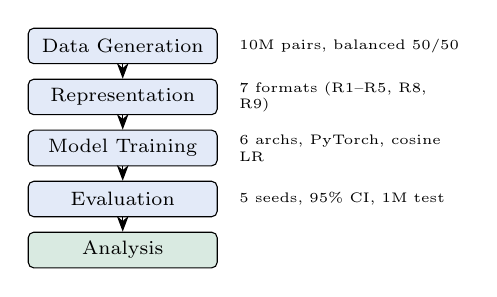
\begin{tikzpicture}[scale=0.72, every node/.style={font=\scriptsize},
  box/.style={draw, rounded corners=2pt, fill=neuralblue!14, minimum width=2.4cm, minimum height=0.45cm, align=center}]
  \node[box] (gen) at (0,3.6) {Data Generation};
  \node[box] (rep) at (0,2.7) {Representation};
  \node[box] (train) at (0,1.8) {Model Training};
  \node[box] (eval) at (0,0.9) {Evaluation};
  \node[box, fill=findinggreen!18] (analysis) at (0,0) {Analysis};
  \draw[-{Stealth[length=2mm]}] (gen) -- (rep);
  \draw[-{Stealth[length=2mm]}] (rep) -- (train);
  \draw[-{Stealth[length=2mm]}] (train) -- (eval);
  \draw[-{Stealth[length=2mm]}] (eval) -- (analysis);

  \node[right=0.15cm, text width=2.8cm, align=left, font=\tiny] at (gen.east) {10M pairs, balanced 50/50};
  \node[right=0.15cm, text width=2.8cm, align=left, font=\tiny] at (rep.east) {7 formats (R1--R5, R8, R9)};
  \node[right=0.15cm, text width=2.8cm, align=left, font=\tiny] at (train.east) {6 archs, PyTorch, cosine LR};
  \node[right=0.15cm, text width=2.8cm, align=left, font=\tiny] at (eval.east) {5 seeds, 95\% CI, 1M test};
\end{tikzpicture}
\end{column}
\end{columns}
\end{frame}

% ==============================================================================
% SLIDE 7: Baseline
% ==============================================================================
\begin{frame}{Baseline: The Distinguishing Cliff}
\small
\begin{columns}[c]
\begin{column}{0.54\textwidth}
\centering
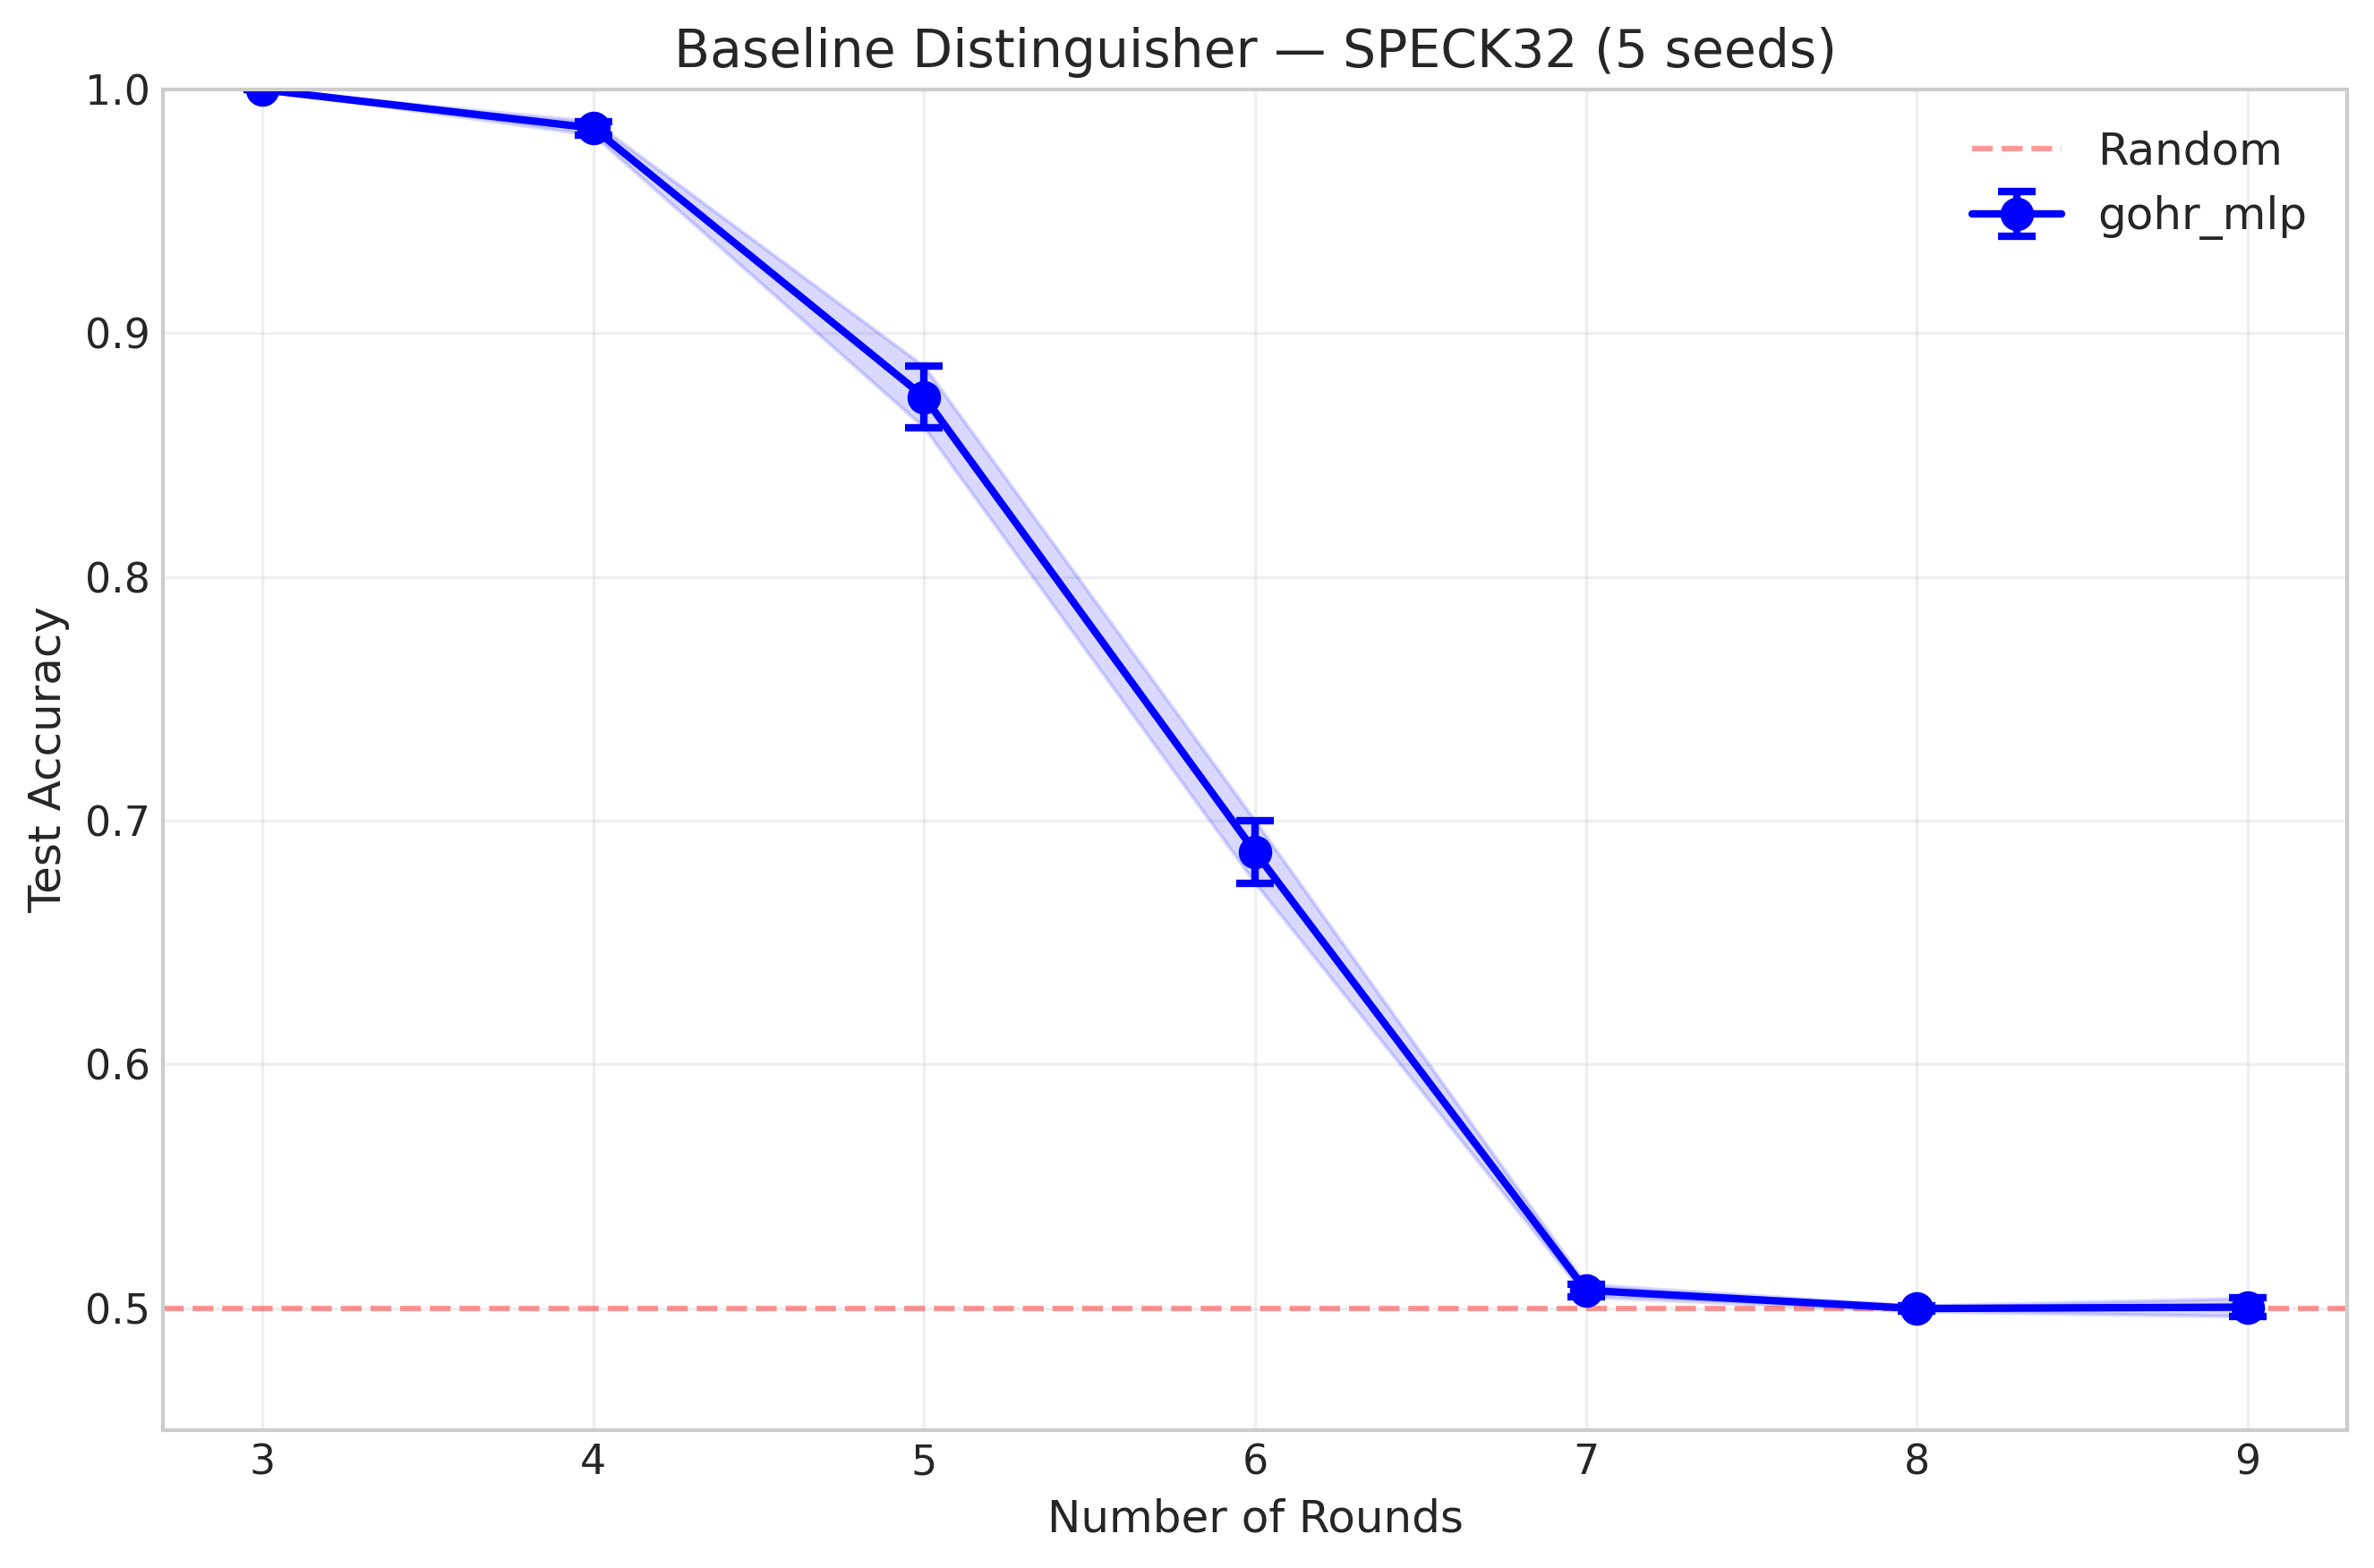
\includegraphics[width=0.9\textwidth]{e01_baseline/e01_speck32.png}
\end{column}
\begin{column}{0.42\textwidth}
\begin{tabular}{@{}cr@{}}
\toprule
\textbf{Rounds} & \textbf{Accuracy} \\
\midrule
3 & 99.99\% \\
4 & 98.42\% \\
5 & 87.38\% \\
6 & 68.72\% \\
7 & 50.73\% \\
\bottomrule
\end{tabular}

Near-perfect at 3--4, random at 7+. Sharp ``cliff'' between rounds 5--7.

Our 87.4\% at R5 vs.\ Gohr's 92.4\% (simpler architecture).
\end{column}
\end{columns}
\end{frame}

% ==============================================================================
% SLIDE 8: Representation Dominates
% ==============================================================================
\begin{frame}{Representation Dominates Architecture}
\small
\begin{columns}[c]
\begin{column}{0.40\textwidth}
\centering

\includegraphics[width=0.85\textwidth]{e02_representation/e02_speck32_r5.png}\\
{\tiny 5 rounds}

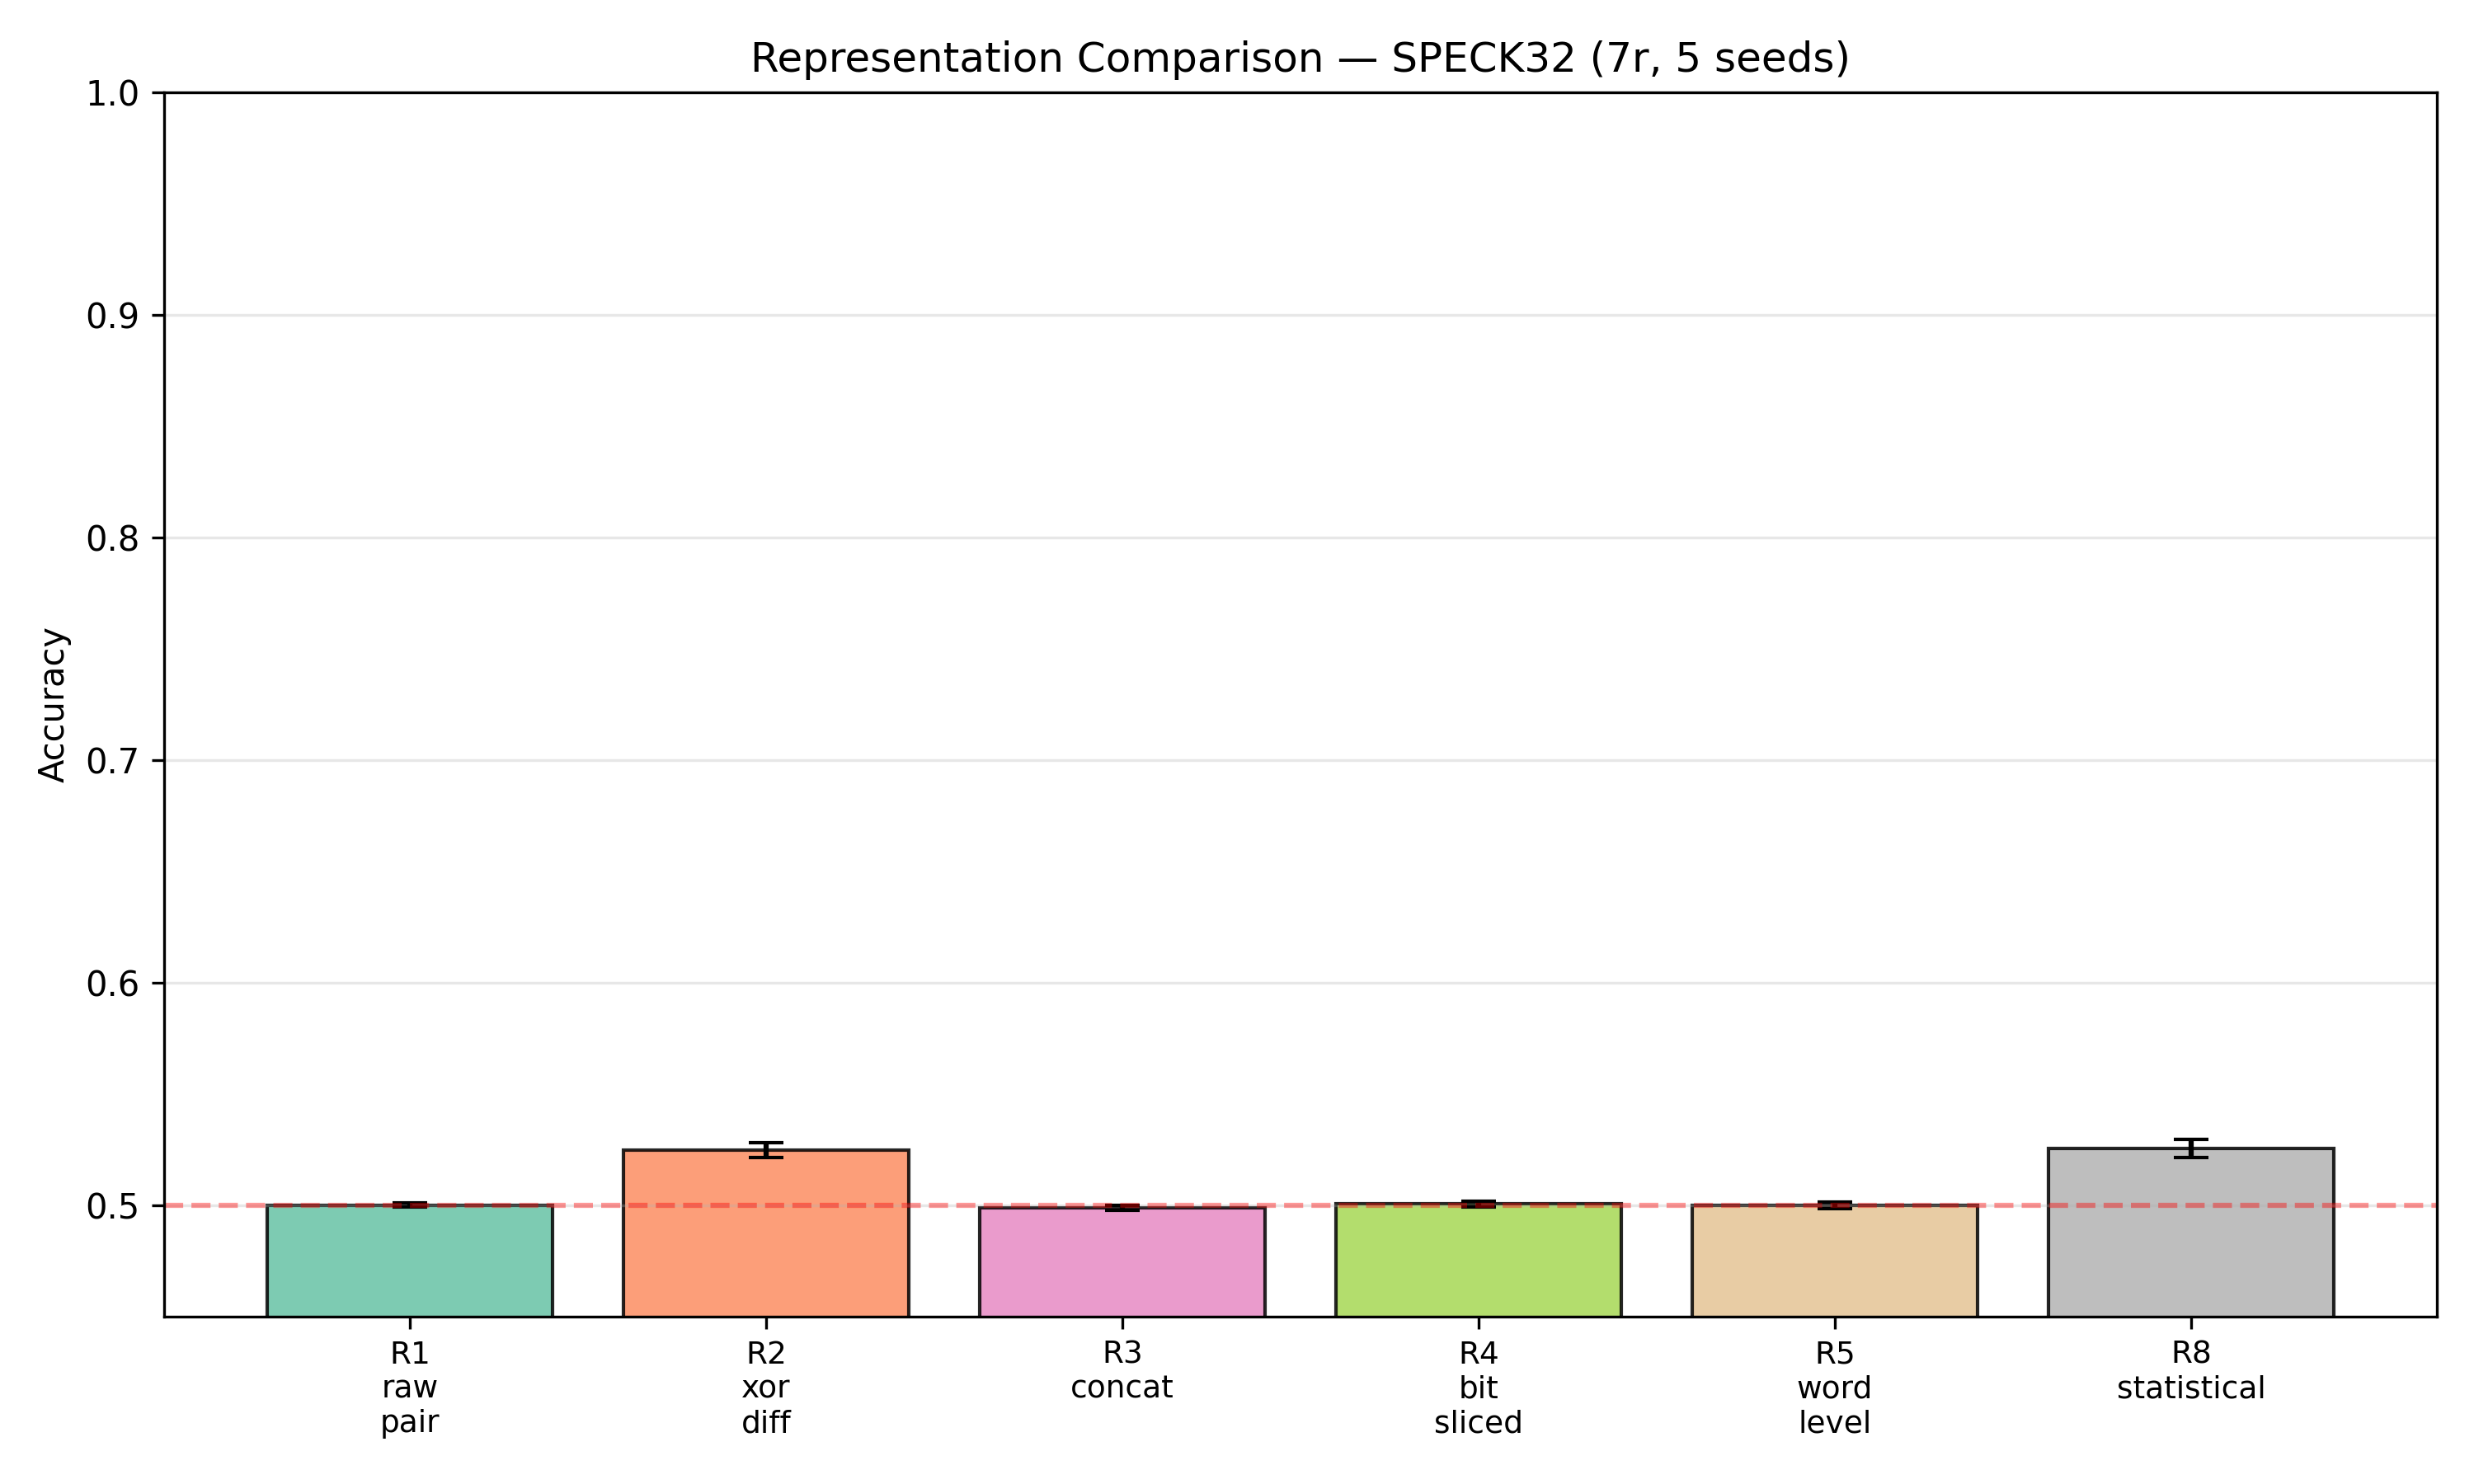
\includegraphics[width=0.85\textwidth]{e02_representation/e02_speck32_r7.png}\\
{\tiny 7 rounds}
\end{column}
\begin{column}{0.56\textwidth}
\textbf{At 5 rounds:}
\begin{itemize}
  \item R2 (XOR diff): \textbf{88.65\%} $\pm$ 0.37
  \item R8 (Statistical): 88.62\% $\pm$ 0.36
  \item R5 (Word-level): 59.80\% $\pm$ 1.60
  \item Representation gap: \textbf{28.85pp}
\end{itemize}

\textbf{At 7 rounds:}
\begin{itemize}
  \item Only R2 (52.5\%) and R8 (52.6\%) retain signal
  \item Everything else collapses to 50\%
\end{itemize}

Architecture spread: only \textbf{3.89pp} (86.1--90.0\%)

\textbf{Takeaway:} \emph{How you preprocess matters far more than which model you use.} XOR diff halves dimensionality at no cost.
\end{column}
\end{columns}
\end{frame}

% ==============================================================================
% SLIDE: Signal Decay Heatmap
% ==============================================================================
\begin{frame}{Signal Decay Heatmap}
\small
\centering
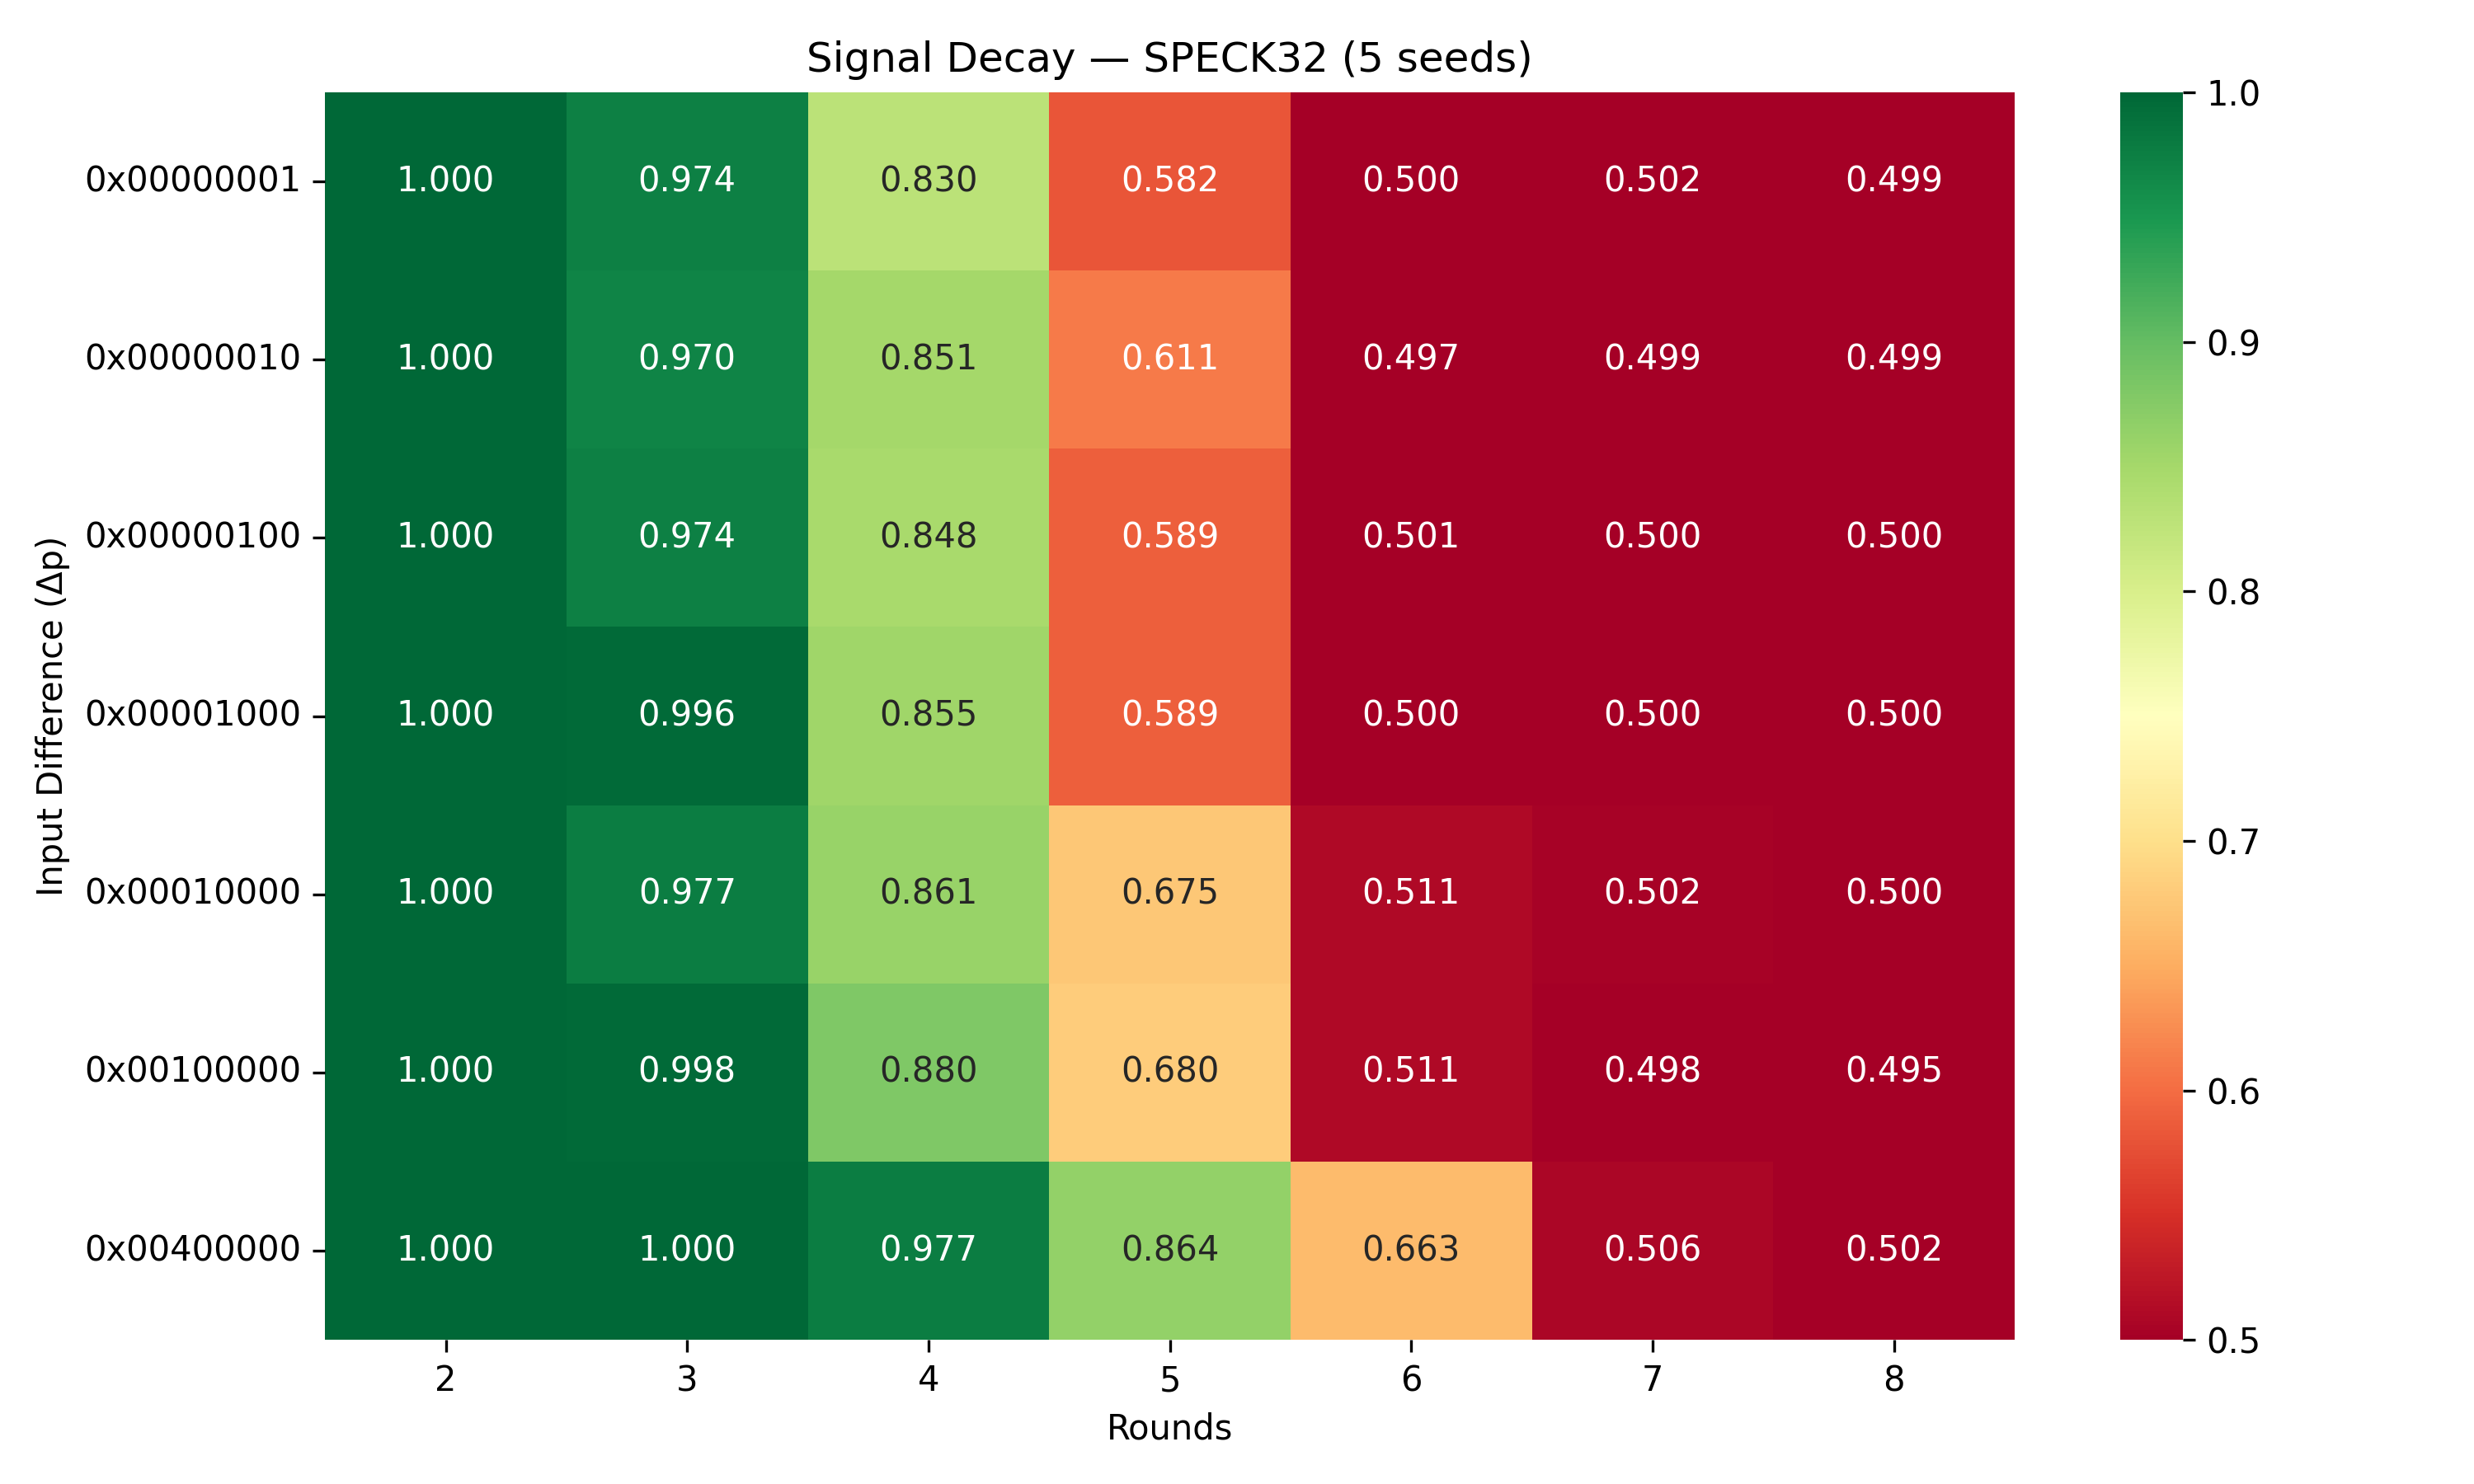
\includegraphics[width=0.55\textwidth]{e07_signal_decay/e07_speck32.png}

{\scriptsize 7 input differences $\times$ 7 round counts. $\Delta P\!=\!\texttt{0x0040\_0000}$: 86.4\% at R5 vs.\ 58.2\% for \texttt{0x01}. All $\to$ 50\% by round 7.}
\end{frame}

% ==============================================================================
% SLIDE 9: Saliency + Invariance
% ==============================================================================
\begin{frame}{The Network Discovers Cipher Structure}
\small
\begin{columns}[c]
\begin{column}{0.50\textwidth}
\centering
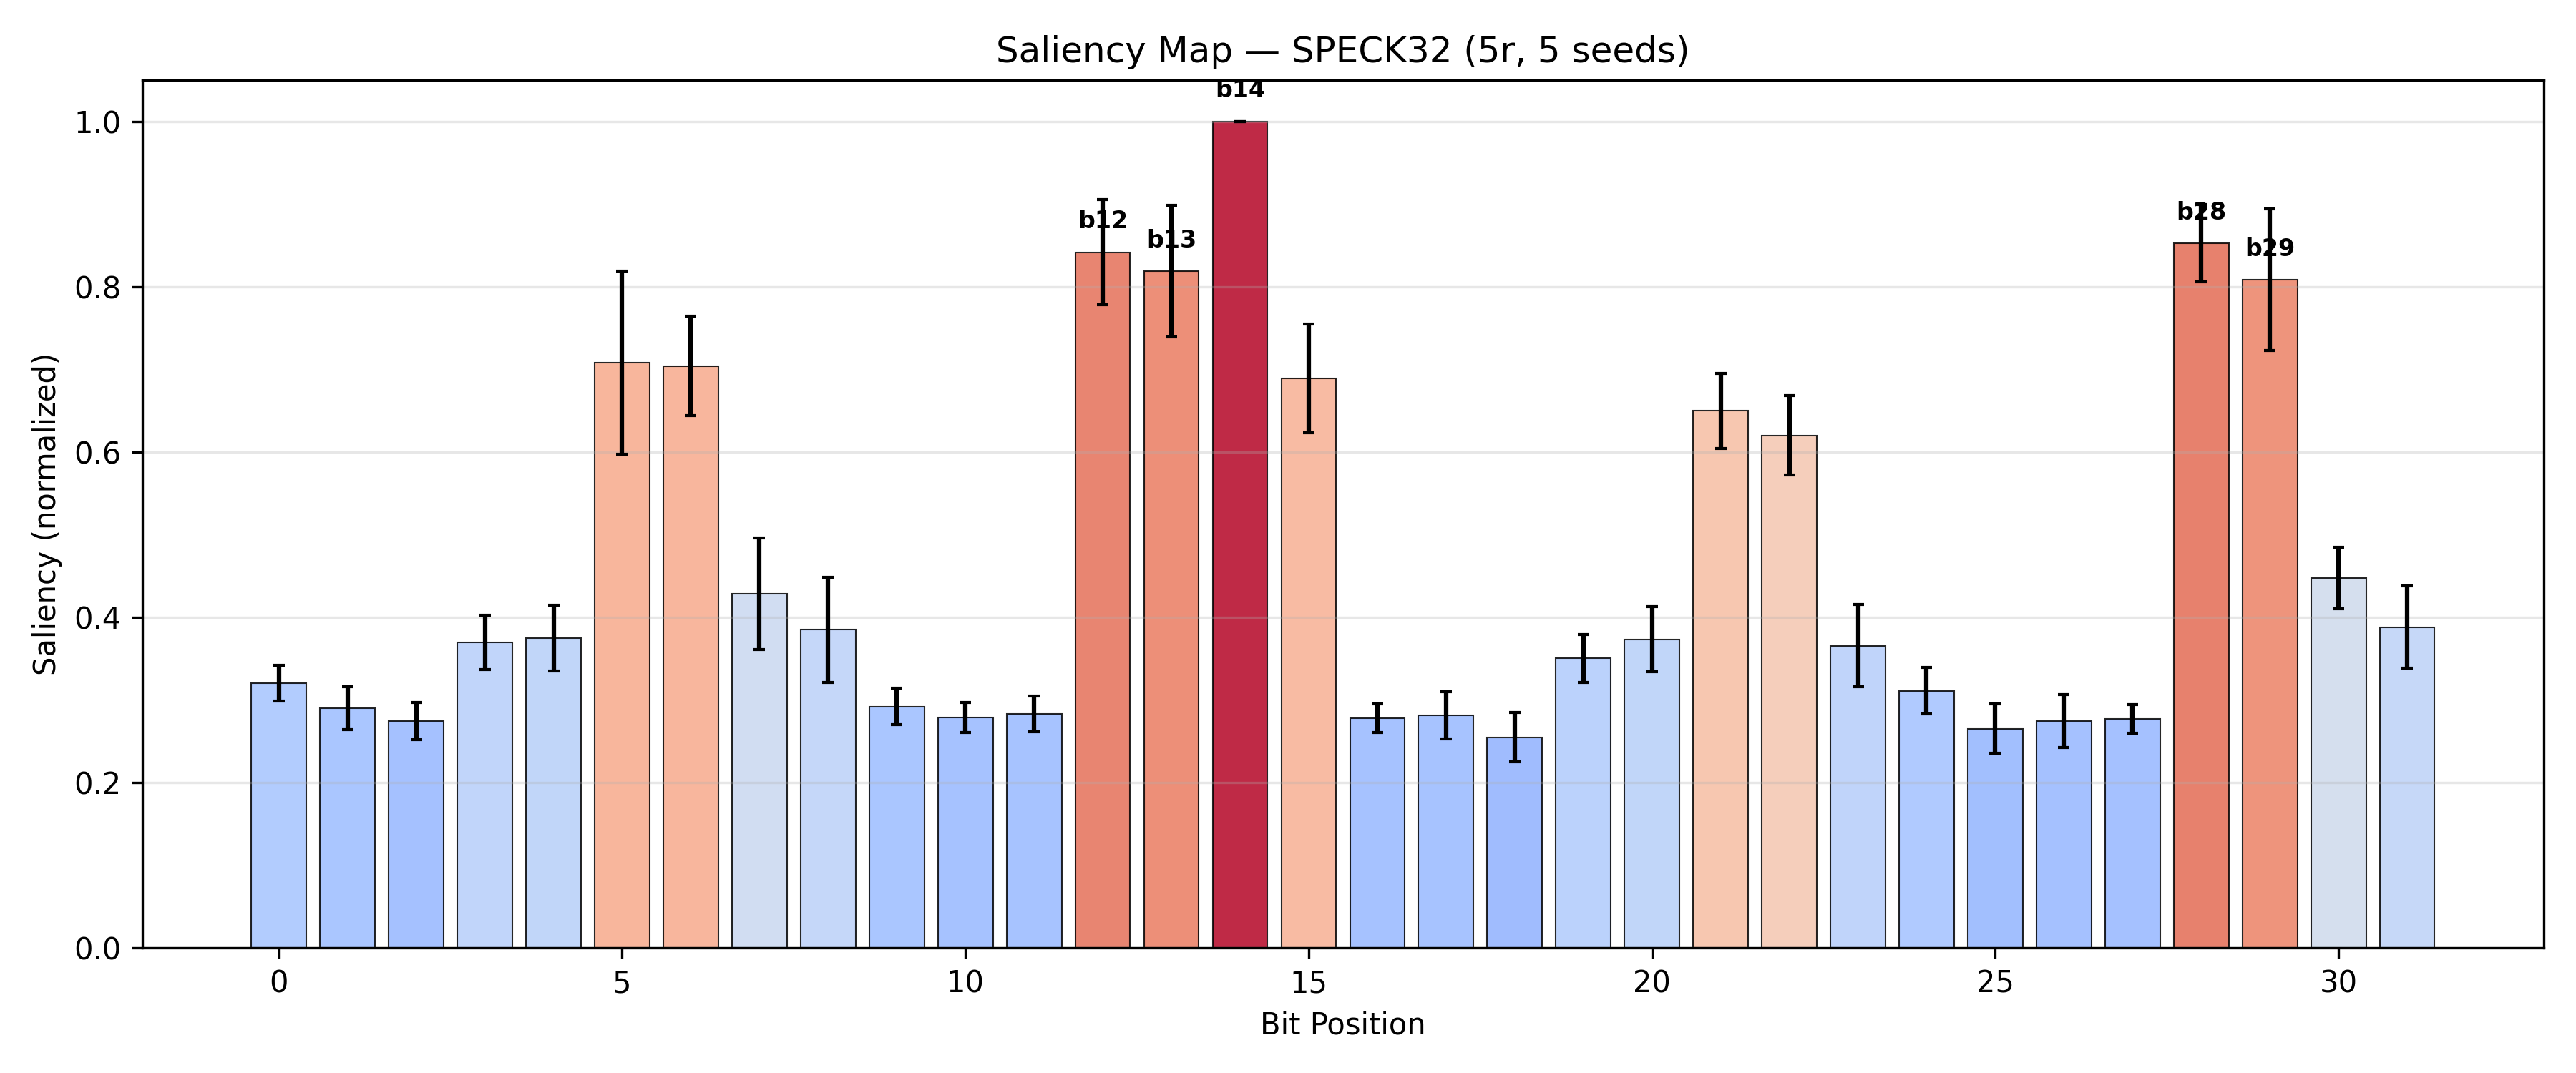
\includegraphics[width=0.9\textwidth]{e08_saliency/e08_speck32_r5.png}\\
{\tiny Gradient saliency across 32 bit positions (5 rounds)}
\end{column}
\begin{column}{0.46\textwidth}
\textbf{Top-5 salient bits:} 14, 28, 12, 13, 29

\begin{itemize}
  \item 16-bit periodicity mirrors SPECK's two-word structure
  \item Bit 14 $\ggg 7$ = bit 7 $\to$ modular addition carry chain
\end{itemize}

\textbf{Invariance test:}\\
Random bit permutation drops accuracy from 87.1\% $\to$ \textbf{50.0\%} ($-$37.1pp).

The model learns \emph{position-specific} features tied to $\alpha\!=\!7$, $\beta\!=\!2$ --- not generic Hamming weight.
\end{column}
\end{columns}
\end{frame}

% ==============================================================================
% SLIDE: Attention Interpretation
% ==============================================================================
\begin{frame}{Attention Interpretation}
\small
\begin{columns}[c]
\begin{column}{0.54\textwidth}
\centering
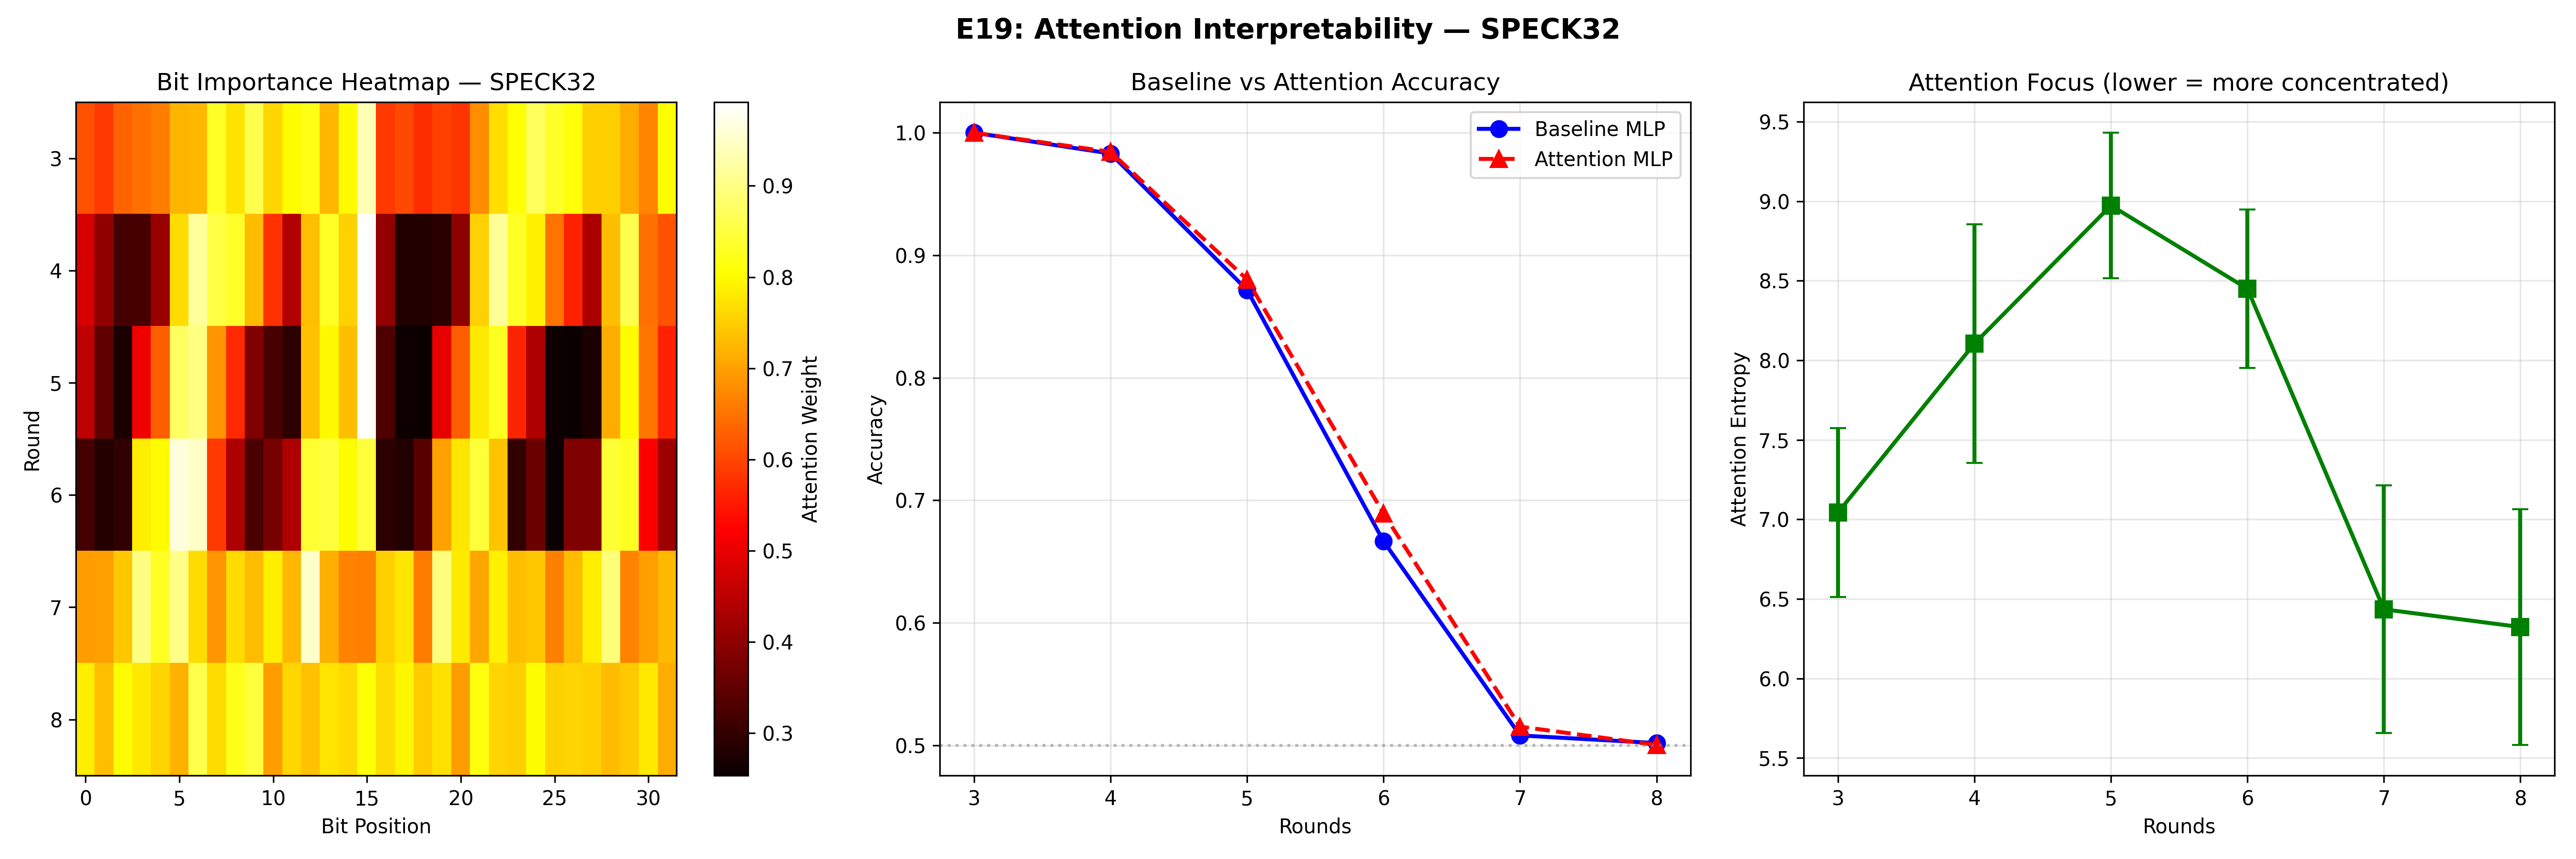
\includegraphics[width=0.9\textwidth]{e19_attention_interp/e19_speck32_attention.png}
\end{column}
\begin{column}{0.43\textwidth}
Attention entropy decreases with round count --- the model \emph{focuses} on fewer bits as the task gets harder.

Aligns with saliency findings.
\end{column}
\end{columns}
\end{frame}

% ==============================================================================
% SLIDE 10: Robustness
% ==============================================================================
\begin{frame}{Robustness Under Noise}
\small
\begin{columns}[c]
\begin{column}{0.54\textwidth}
\centering
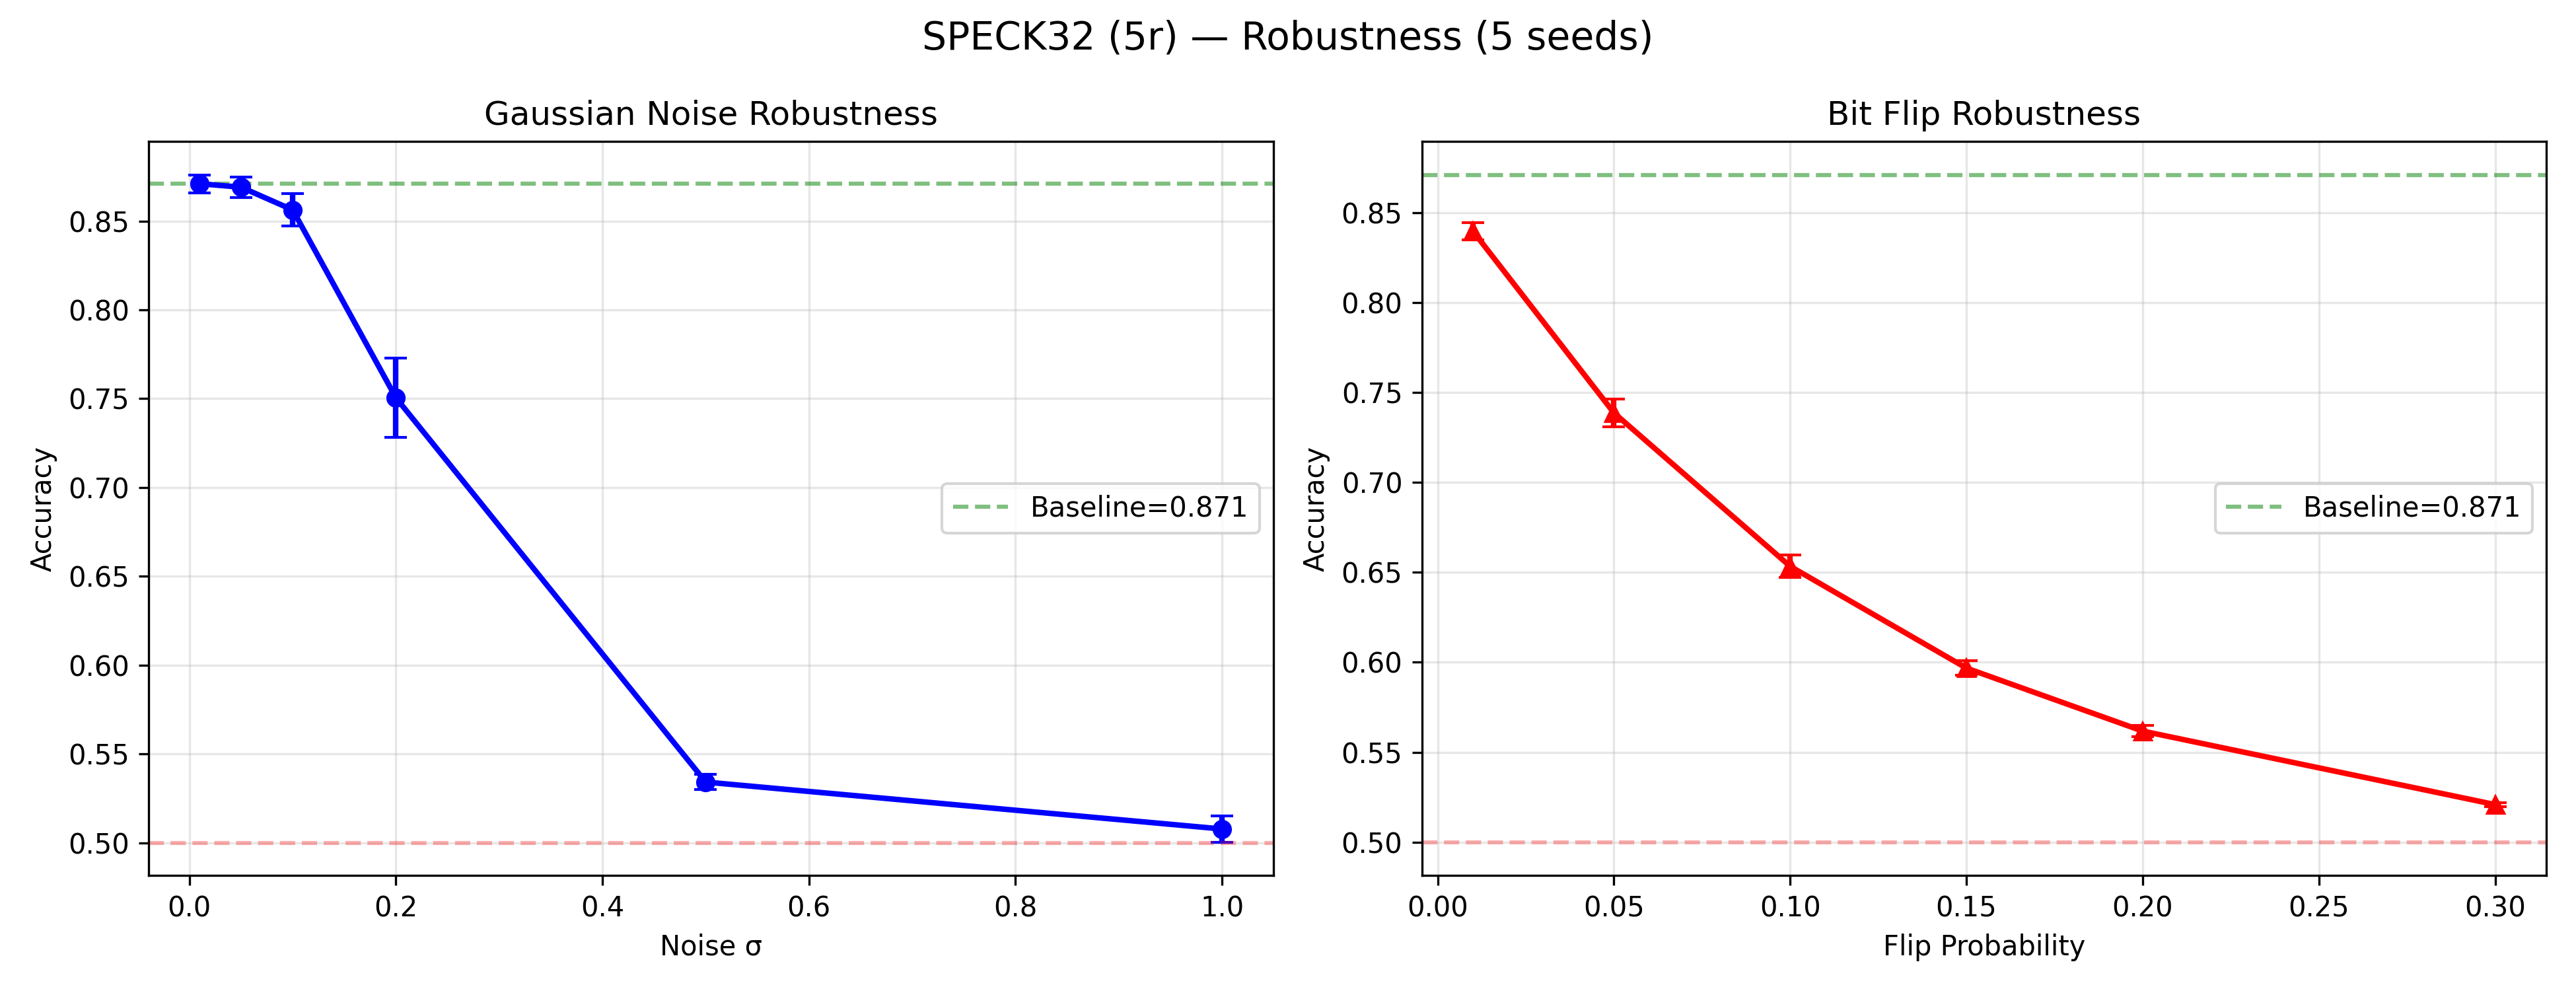
\includegraphics[width=0.9\textwidth]{e04_robustness/e04_speck32_r5.png}
\end{column}
\begin{column}{0.42\textwidth}
\begin{tabular}{@{}cccc@{}}
\toprule
\multicolumn{2}{c}{\textbf{Gaussian}} & \multicolumn{2}{c}{\textbf{Bit Flip}} \\
\cmidrule(lr){1-2} \cmidrule(lr){3-4}
$\sigma$ & Acc & $p$ & Acc \\
\midrule
0.05 & 86.9\% & 0.01 & 84.0\% \\
0.10 & 85.6\% & 0.05 & 73.9\% \\
0.20 & 75.1\% & 0.10 & 65.3\% \\
0.50 & 53.4\% & 0.20 & 56.2\% \\
\bottomrule
\end{tabular}

\begin{itemize}
  \item Gaussian: tolerant up to $\sigma\!=\!0.1$
  \item Bit flips far more destructive --- even 1\% $\Rightarrow$ $-$3.1pp
  \item \textbf{Practical limit:} BER $<$ 5\%
\end{itemize}
\end{column}
\end{columns}
\end{frame}

% ==============================================================================
% SLIDE 11: Markov Validated
% ==============================================================================
\begin{frame}{Markov Assumption: Validated}
\small
\begin{columns}[c]
\begin{column}{0.48\textwidth}
\centering
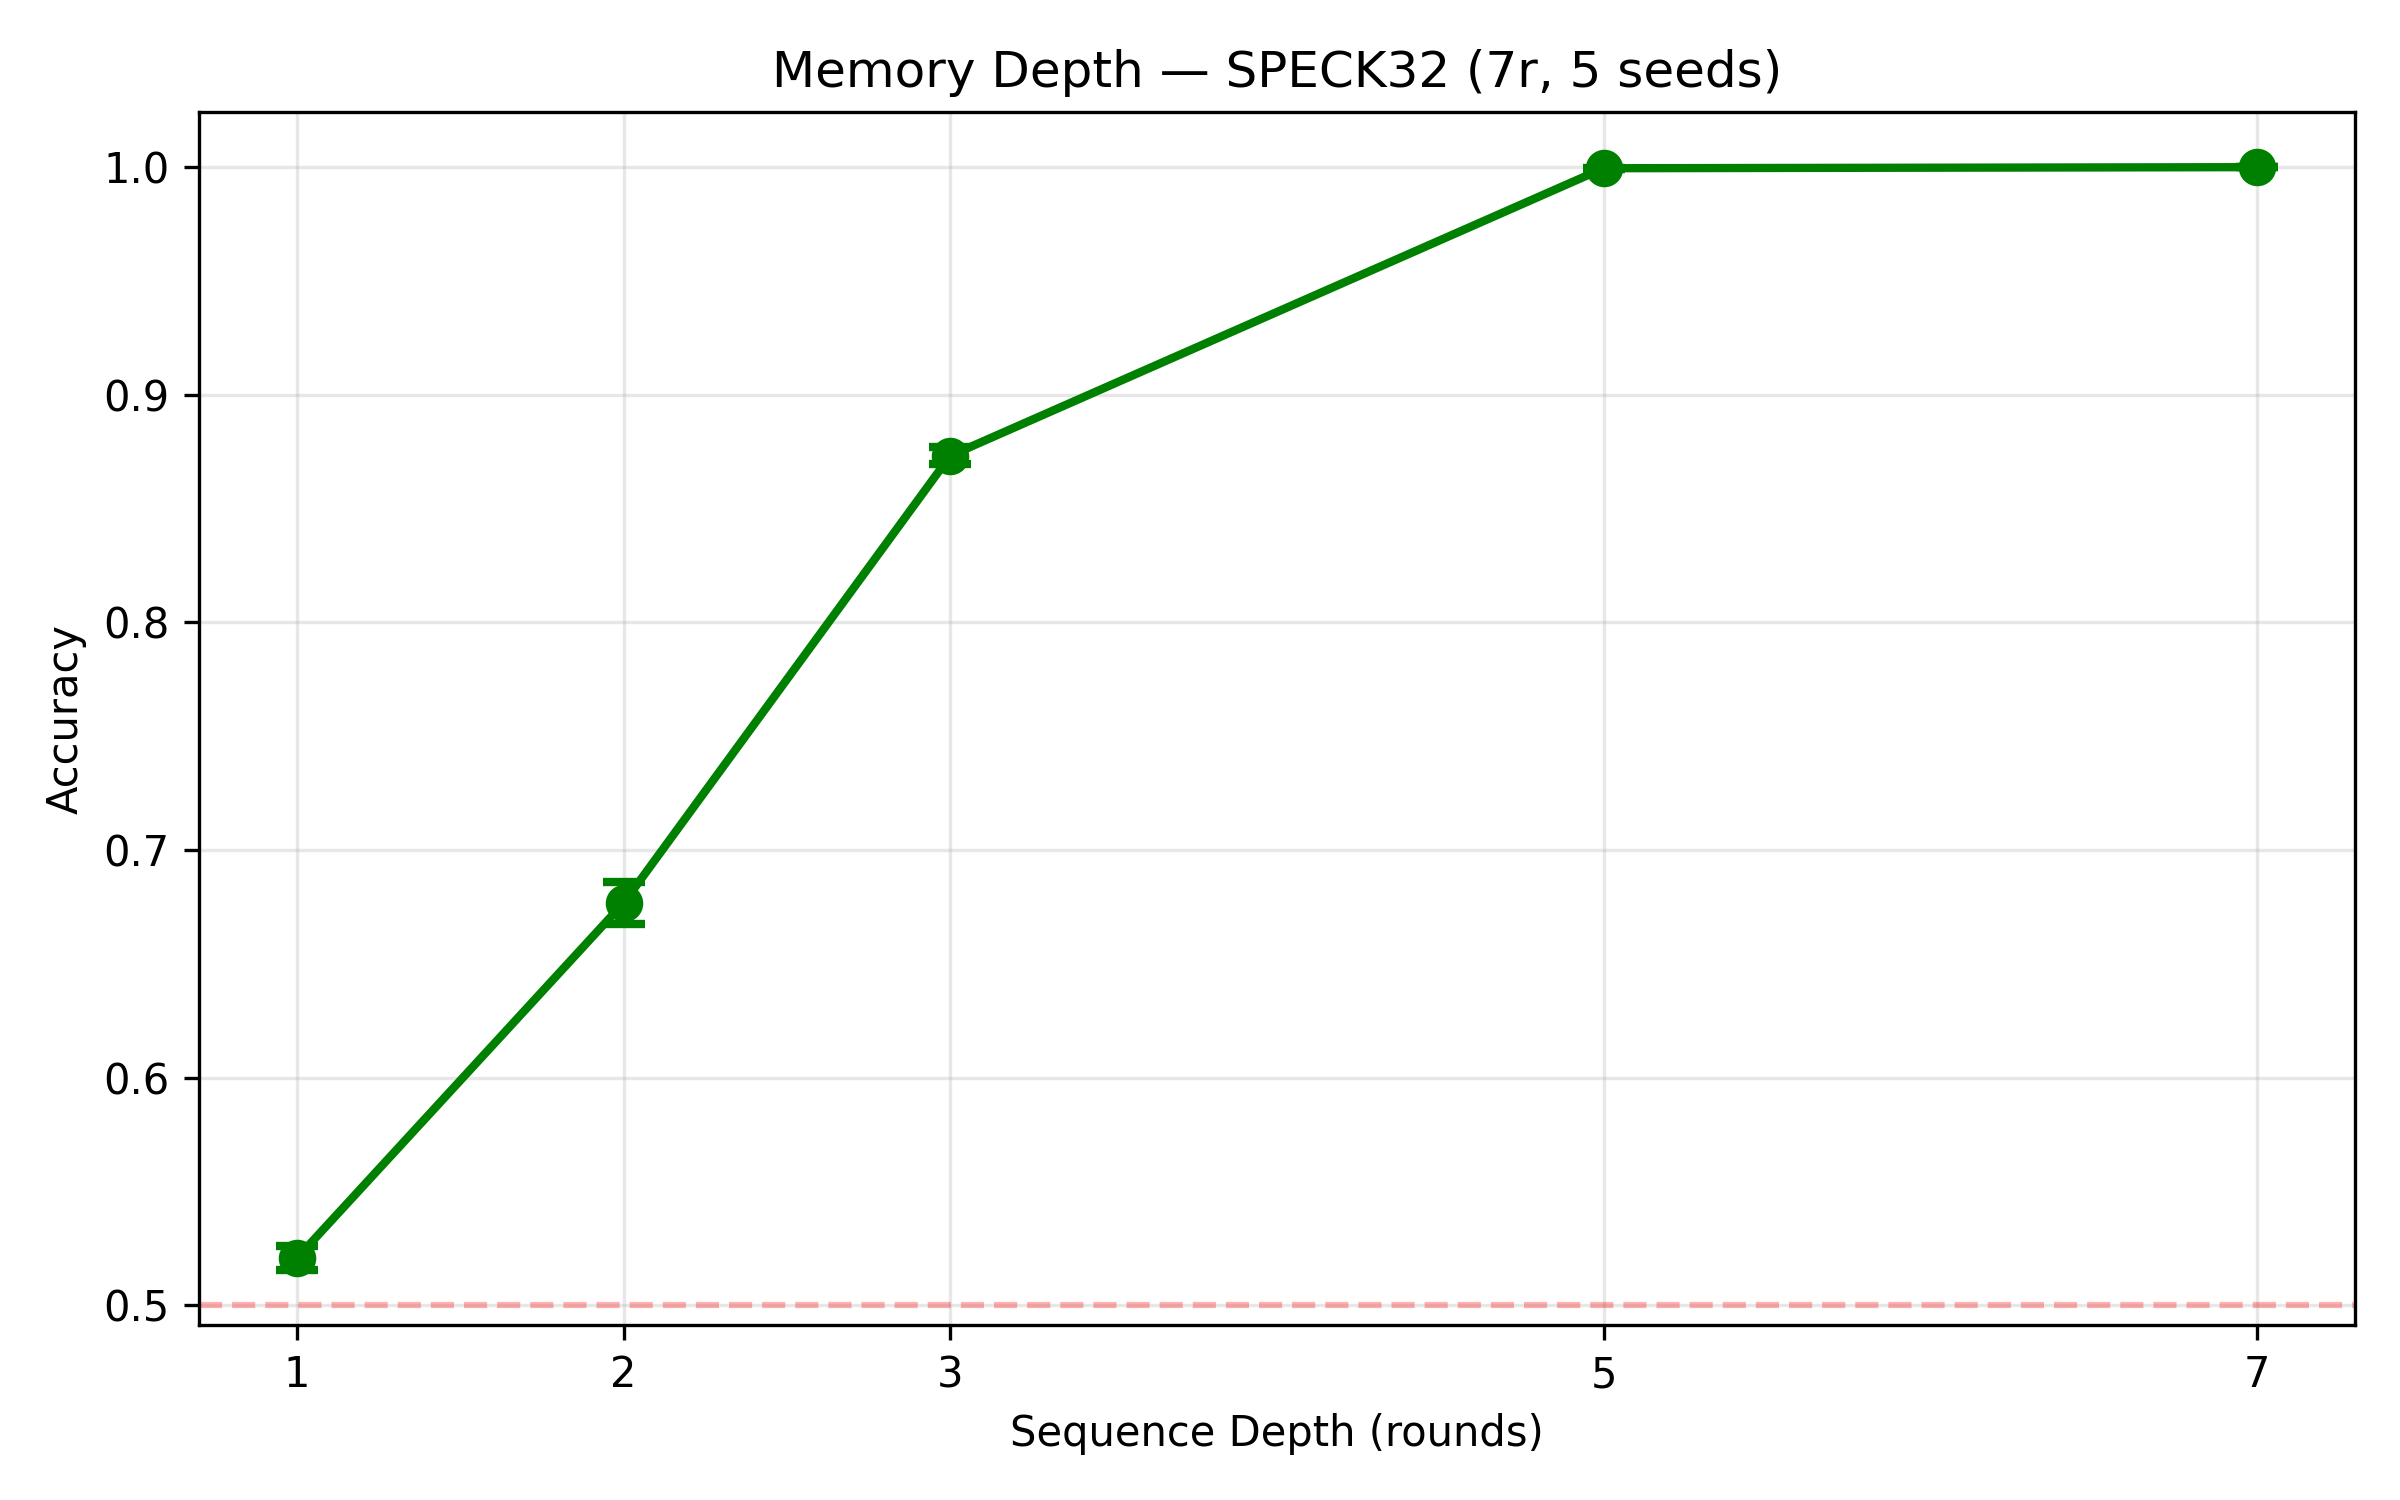
\includegraphics[width=0.85\textwidth]{e05_markov_depth/e05_speck32_r7.png}

{\scriptsize \textbf{Depth analysis} (7-round target)\\
$d\!=\!1$: 52\%~~$d\!=\!3$: 87\%~~$d\!=\!7$: 100\%}
\end{column}
\begin{column}{0.48\textwidth}
\centering
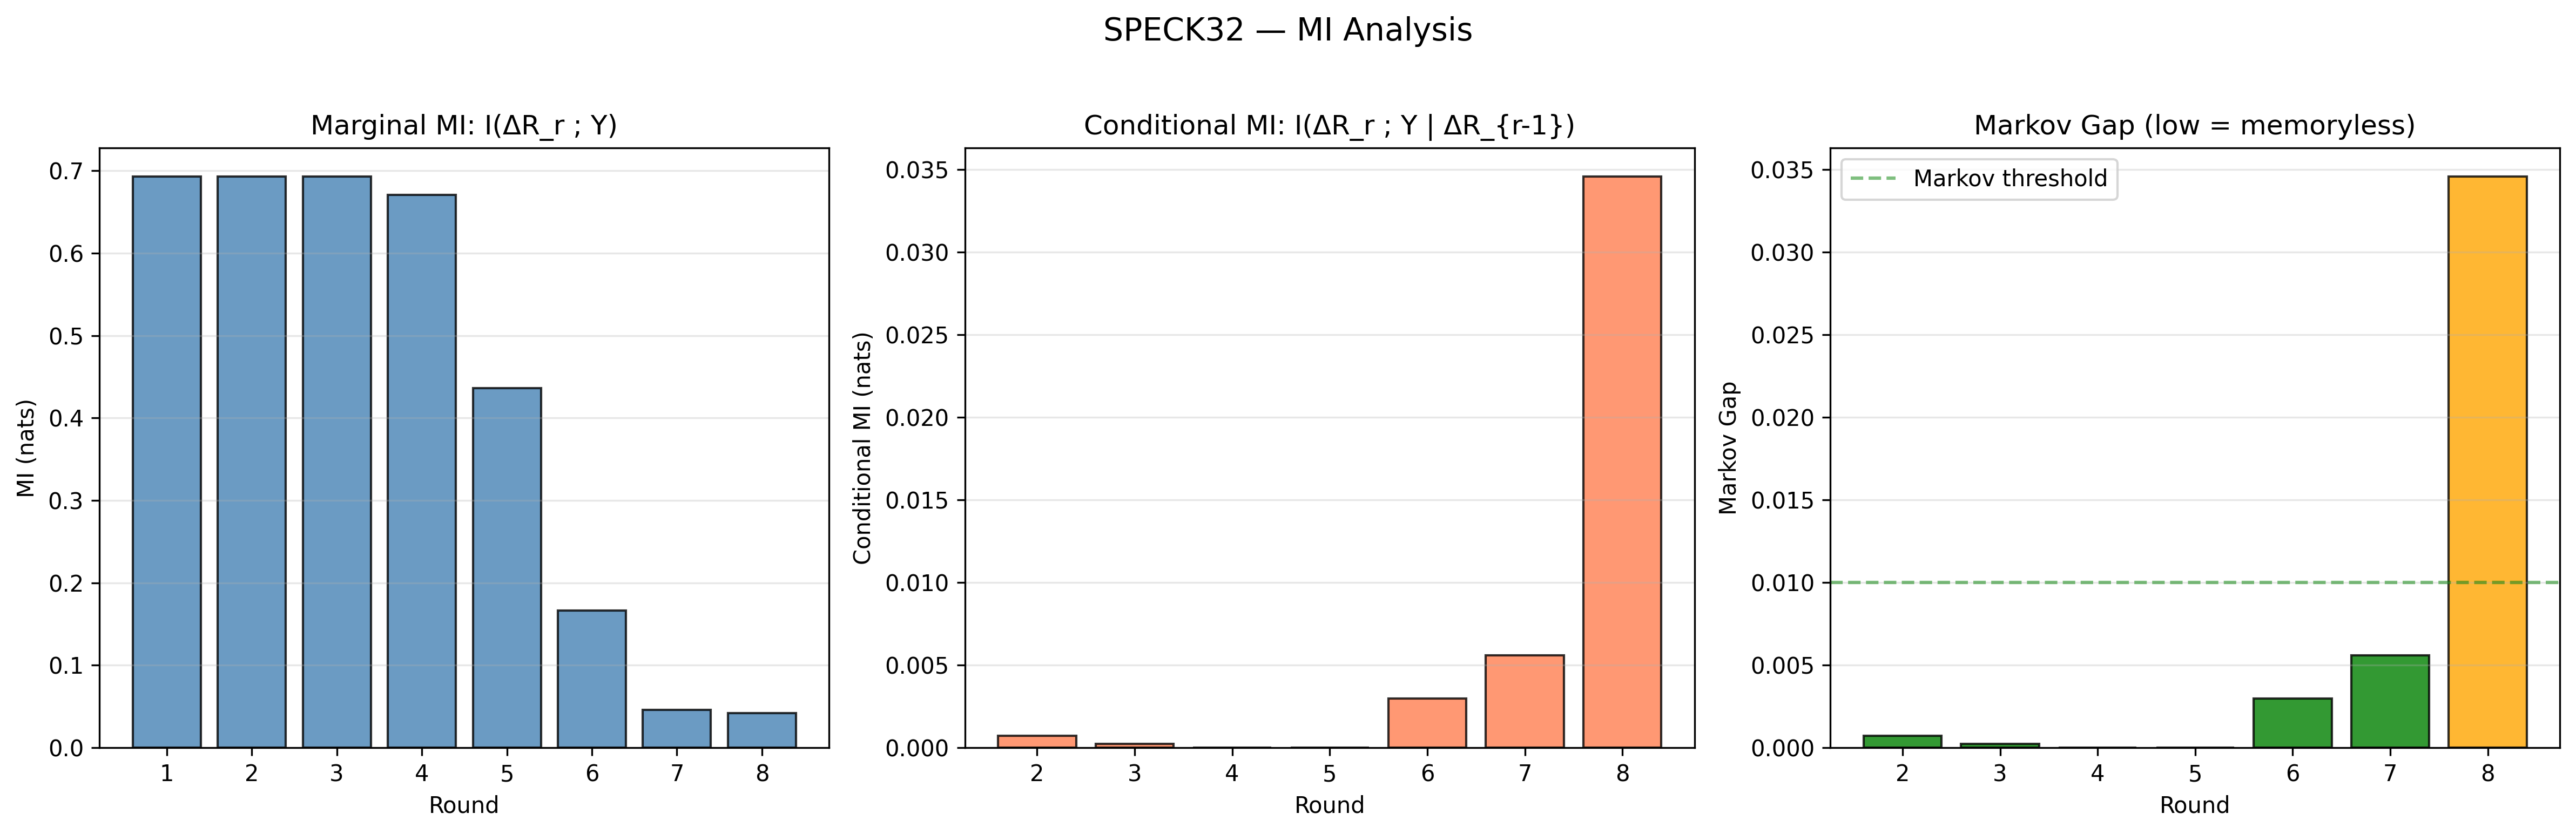
\includegraphics[width=0.85\textwidth]{e06_conditional_mi/e06_speck32.png}

{\scriptsize \textbf{Conditional MI} $\approx 0$ at all\\
round transitions --- no residual dependency.}
\end{column}
\end{columns}

\vspace{0.15cm}
\centering
\textbf{Three independent methods agree:} depth analysis, MINE estimation, and generative modeling all confirm the Markov assumption holds for SPECK32.
\end{frame}

% ==============================================================================
% SLIDE 13: Latent Space + VAE
% ==============================================================================
\begin{frame}{Latent Space \& Generative Markov Validation}
\small
\begin{columns}[c]
\begin{column}{0.54\textwidth}
\centering

\includegraphics[width=\textwidth]{e16_generative_markov/e16_speck32_latent.png}
\end{column}
\begin{column}{0.43\textwidth}
\textbf{Variational Autoencoder (VAE) Latent Space:}

Reveals well-separated, clustered representations corresponding directly to the underlying cipher state (real vs.\ random). 

\vspace{0.2cm}
Validates that generated ciphertext differences maintain the exact structural properties of true differentials.
\end{column}
\end{columns}
\end{frame}

% ==============================================================================
% SLIDE 12: Neural vs Classical + Automated Search
% ==============================================================================
\begin{frame}{Neural vs.\ Classical \& Automated Search}
\small
\begin{columns}[c]
\begin{column}{0.48\textwidth}
\centering
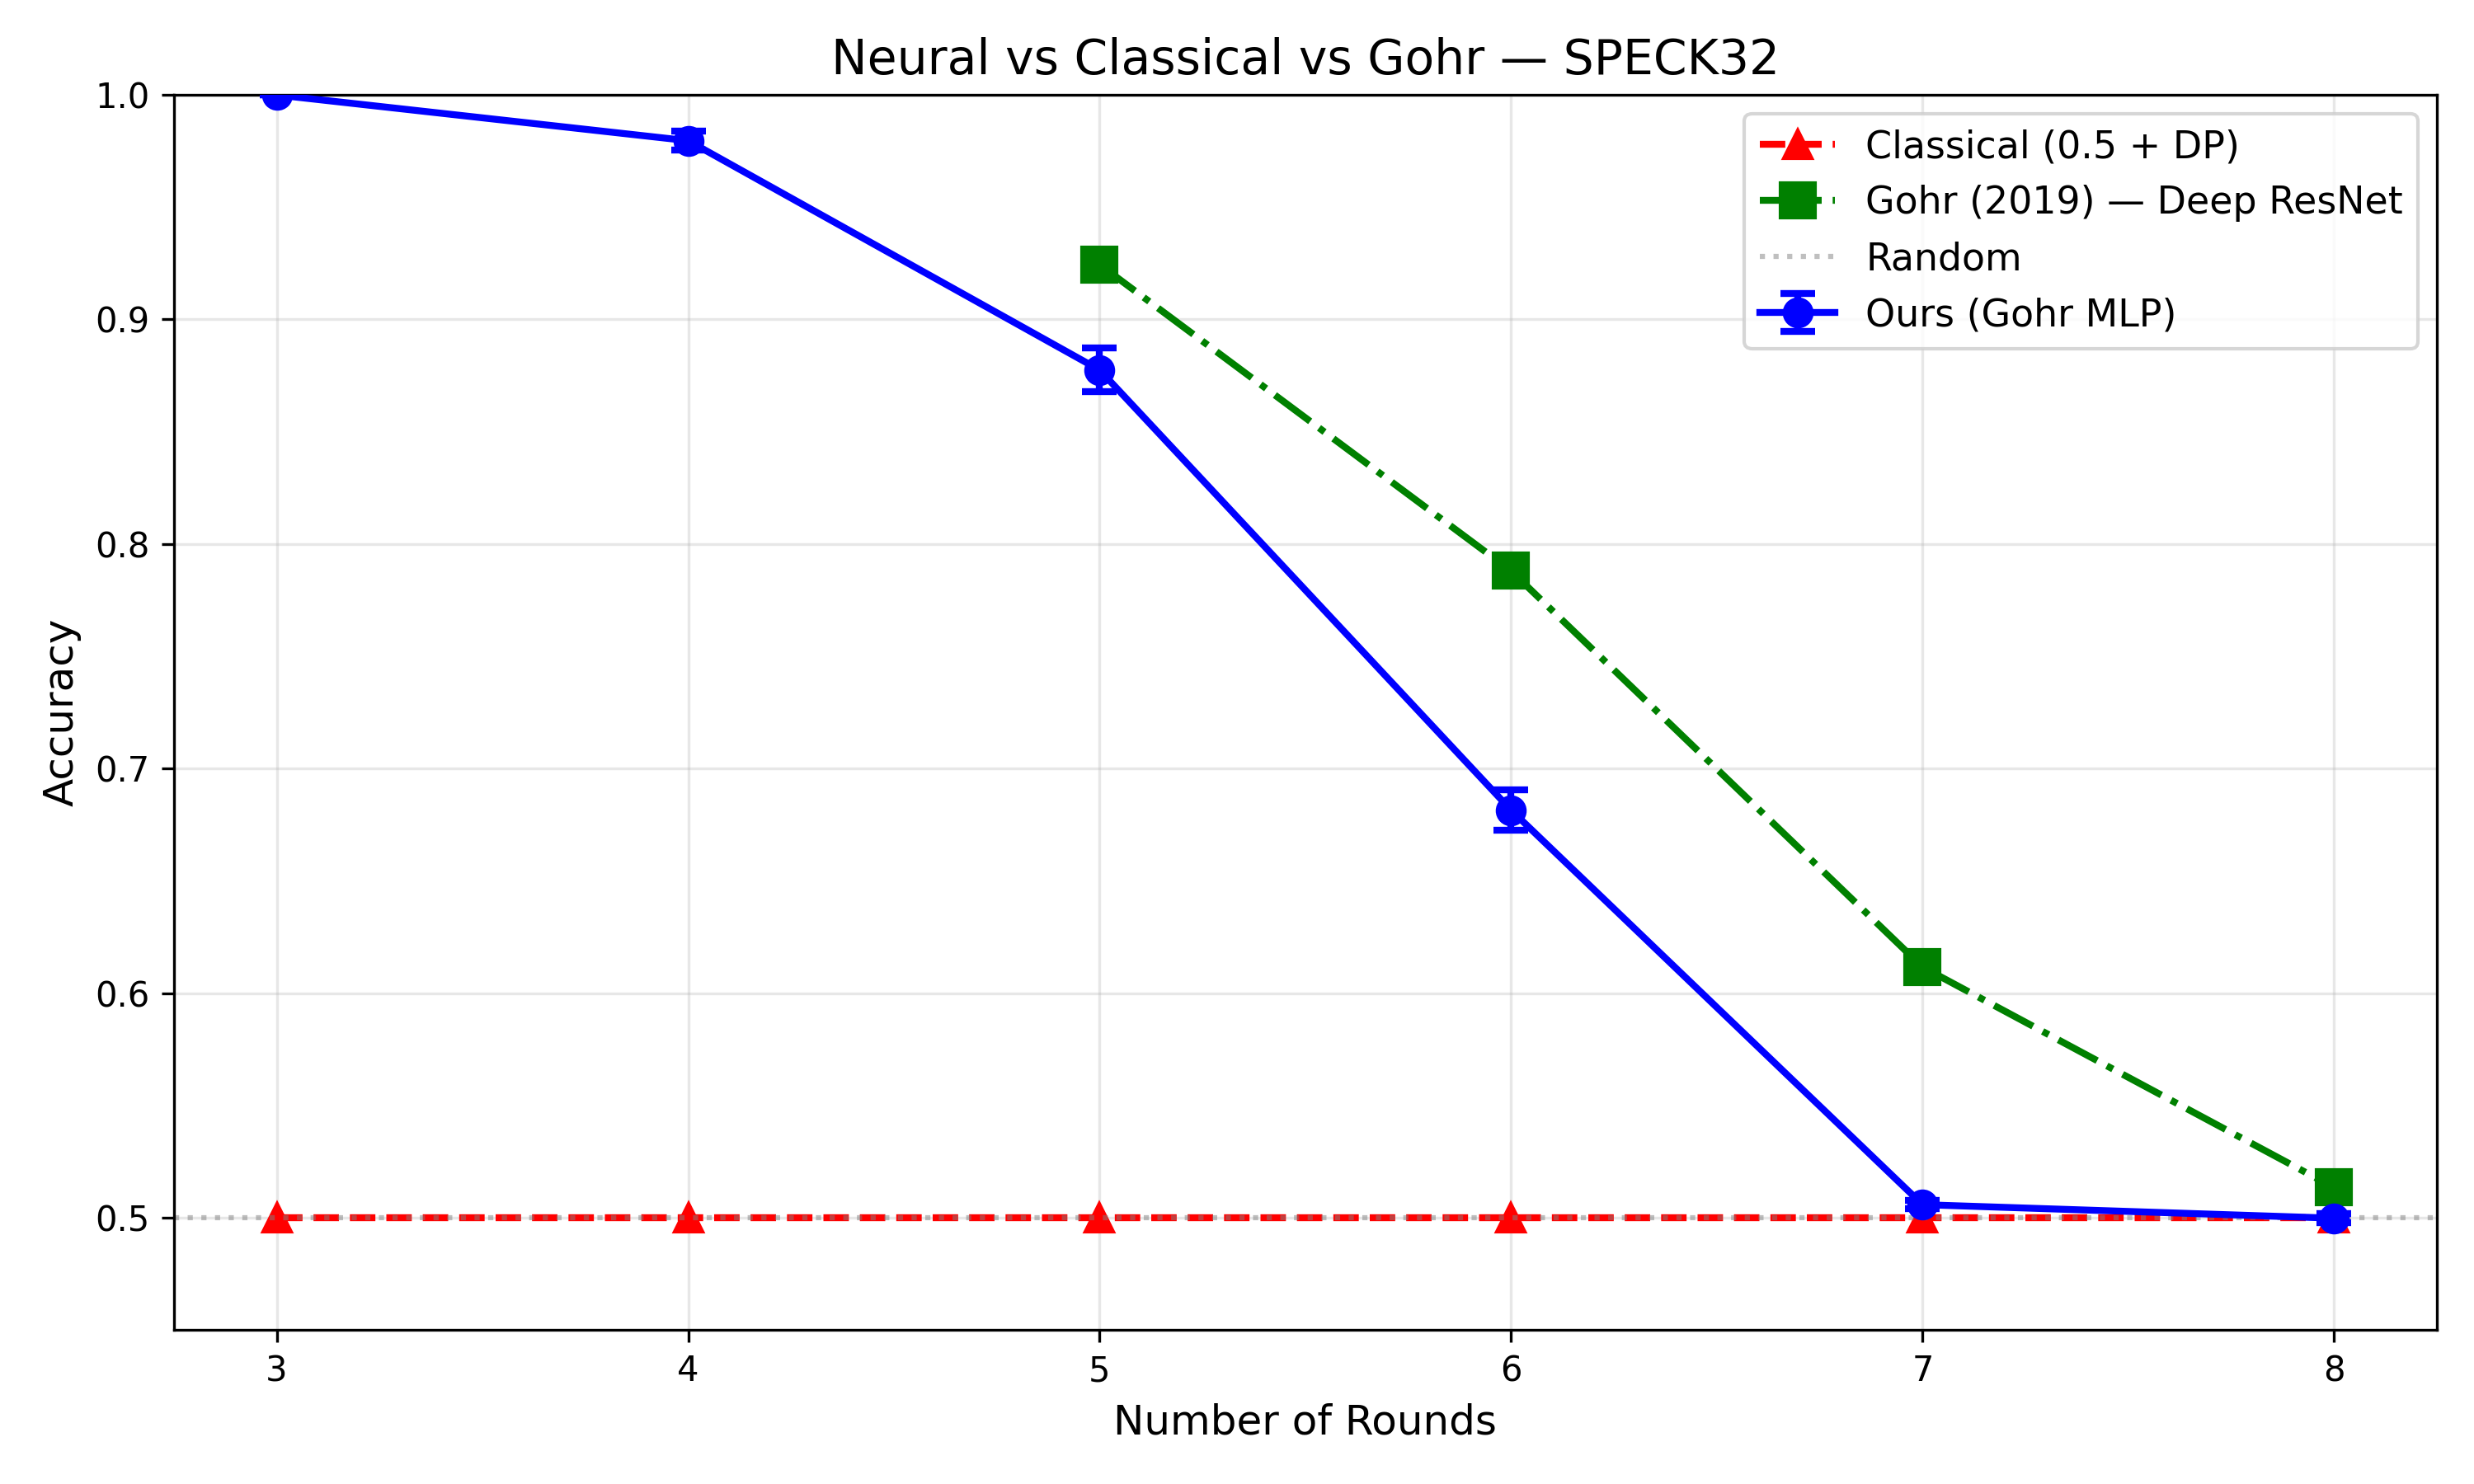
\includegraphics[width=0.85\textwidth]{e11_classical/e11_speck32.png}

{\scriptsize Classical sample-based DP: $<\!2^{-16}$\\(undetectable from finite samples).\\
Neural: 87.8\% at R5, 68.2\% at R6.}
\end{column}
\begin{column}{0.48\textwidth}
\centering
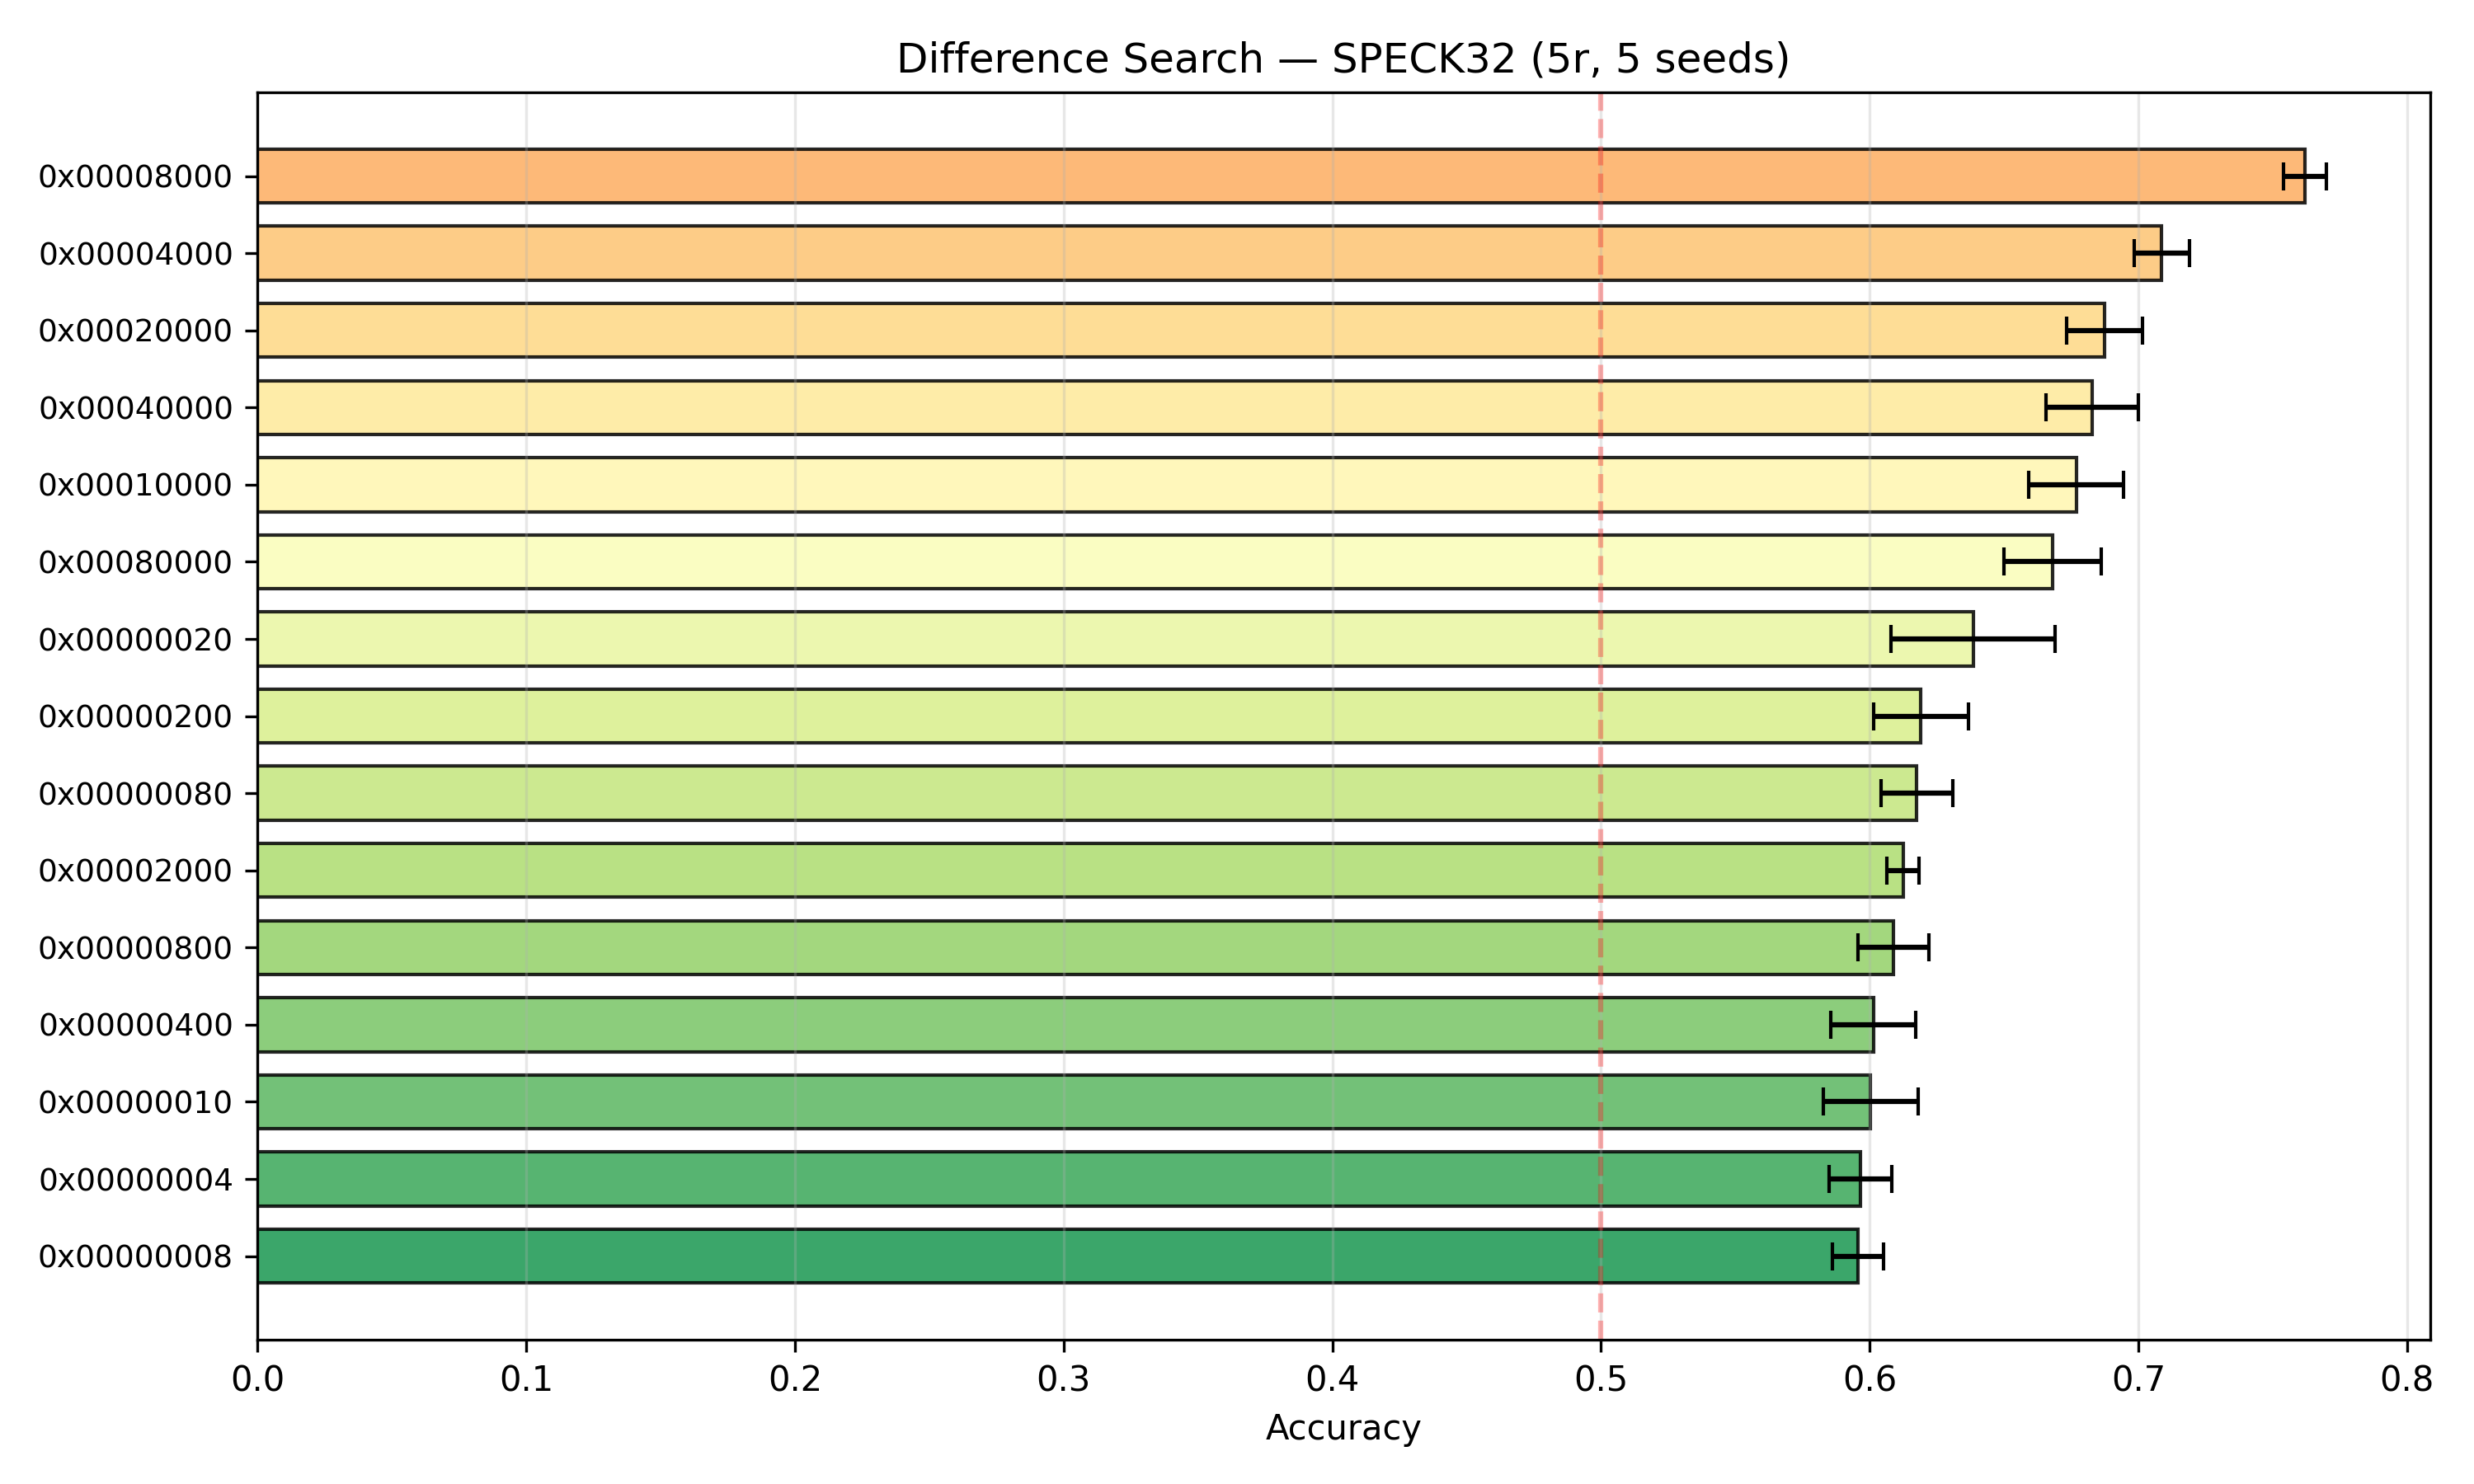
\includegraphics[width=0.85\textwidth]{e10_diff_search/e10_speck32_r5.png}

{\scriptsize Best single-bit $\Delta P$: \texttt{0x8000} at 76.2\%.\\
Worst: \texttt{0x01} at 57.8\%.\\
Top diffs cluster in bits 14--19.}
\end{column}
\end{columns}
\end{frame}

% ==============================================================================
% SLIDE: RL-Based Differential Search
% ==============================================================================
\begin{frame}{RL-Based Differential Search}
\small
\begin{columns}[c]
\begin{column}{0.54\textwidth}
\centering

\includegraphics[width=0.9\textwidth]{e18_diff_search_r3/e18_speck32_diff_search.png}
\end{column}
\begin{column}{0.43\textwidth}
At 3 rounds: RL discovers \texttt{0x0010\_2000} at \textbf{84.96\%} (known-optimal: 86.63\%).

\vspace{0.2cm}
At 5 rounds: insufficient gradient signal for RL exploration.
\end{column}
\end{columns}
\end{frame}


% ==============================================================================
% SLIDE 14: Architecture & Data Efficiency
% ==============================================================================
\begin{frame}{Architecture \& Data Efficiency}
\small
\begin{columns}[c]
\begin{column}{0.48\textwidth}
\centering
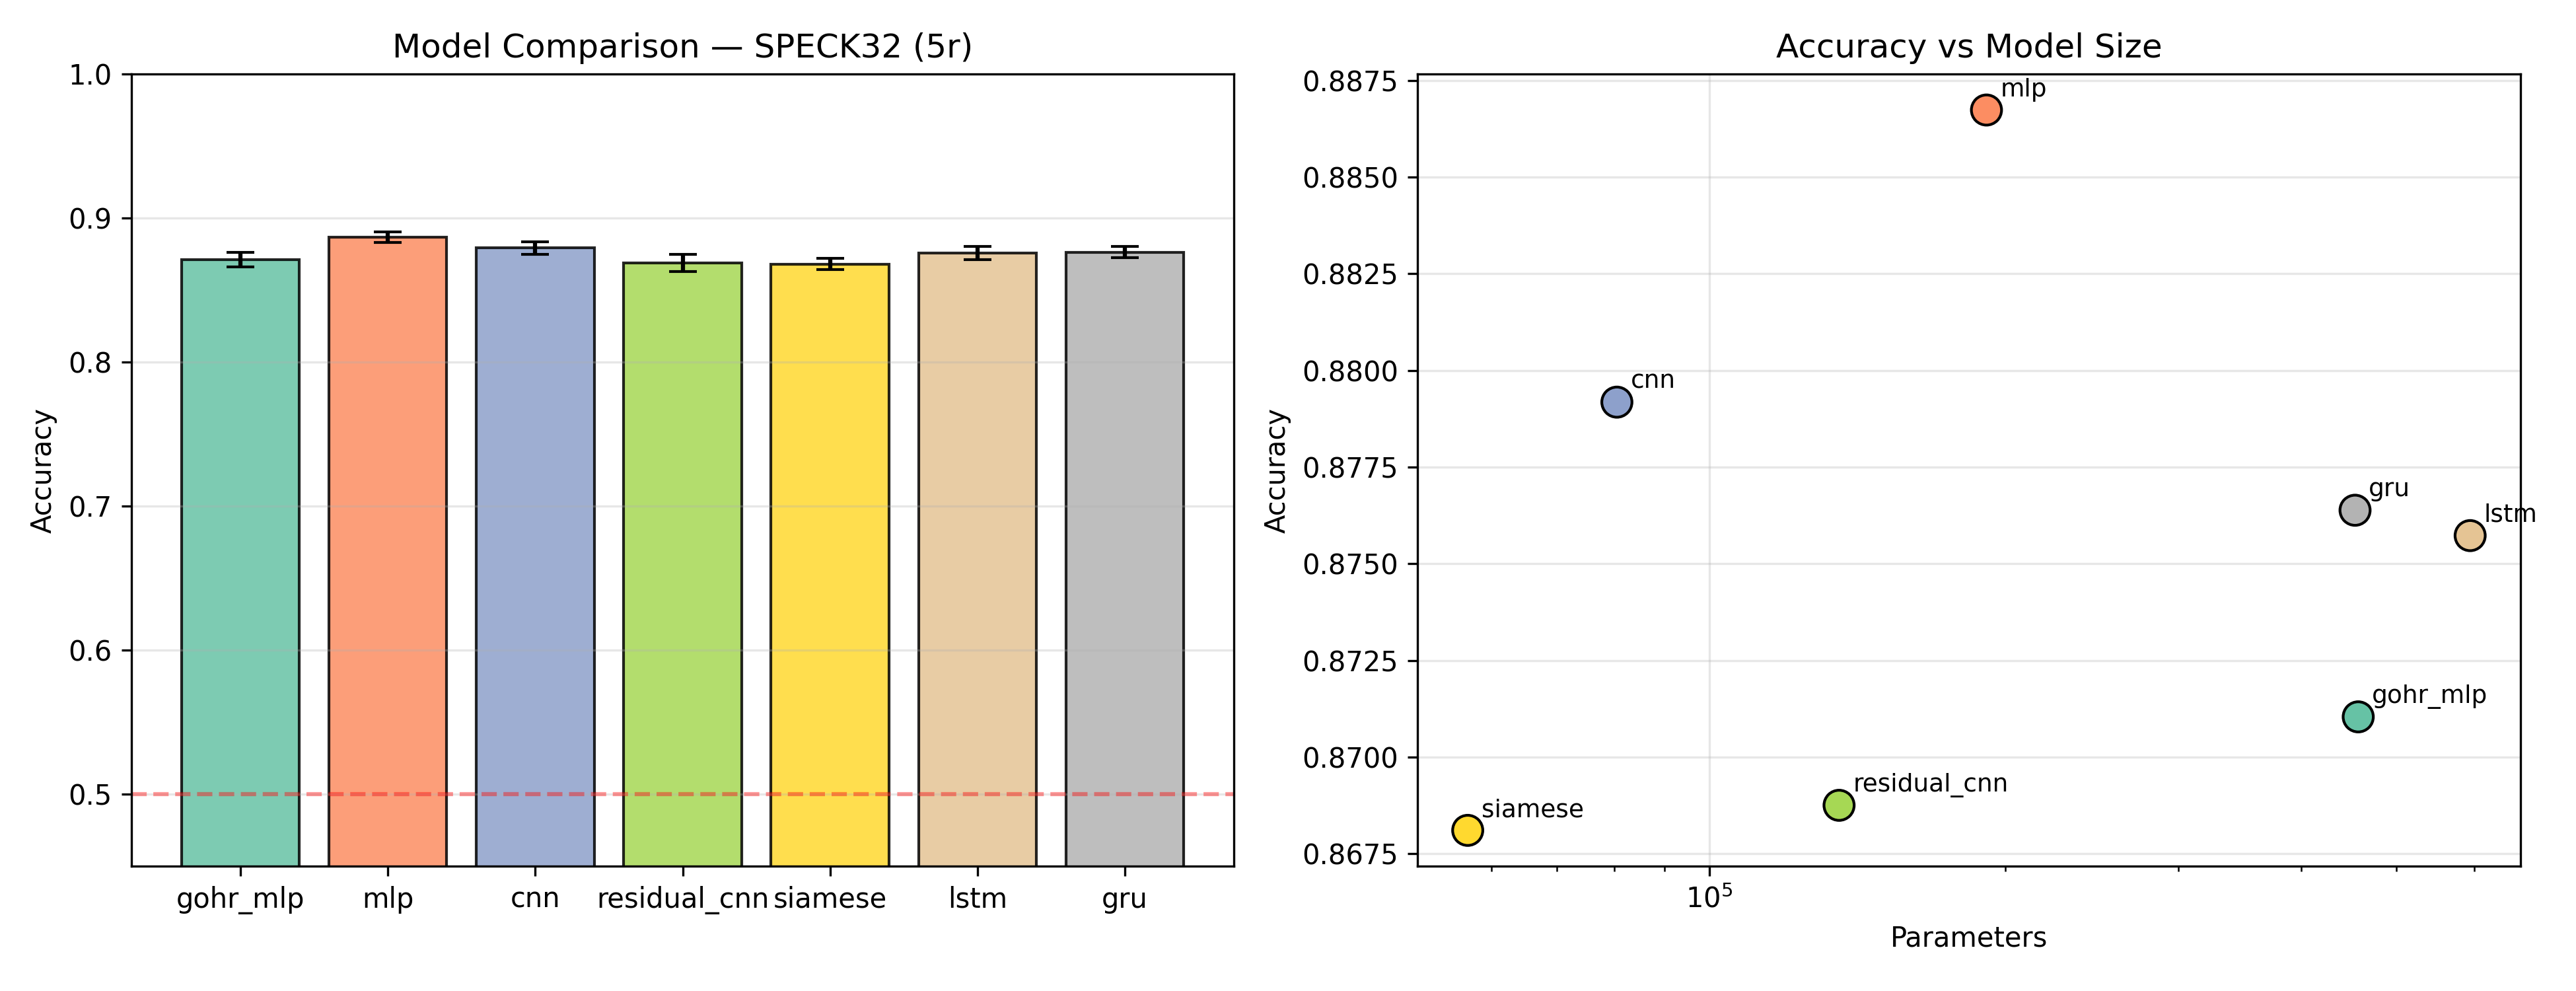
\includegraphics[width=0.85\textwidth]{e13_model_comparison/e13_speck32_r5.png}

\begin{tabular}{@{}lrr@{}}
\toprule
\textbf{Model} & \textbf{Params} & \textbf{Acc} \\
\midrule
LSTM & 594K & \textbf{90.0\%} \\
MLP & 191K & 88.5\% \\
CNN & 81K & 88.4\% \\
Gohr MLP & 457K & 86.1\% \\
\bottomrule
\end{tabular}

{\scriptsize CNN: $7.3\times$ smaller, only $-$1.6pp.}
\end{column}
\begin{column}{0.48\textwidth}
\centering
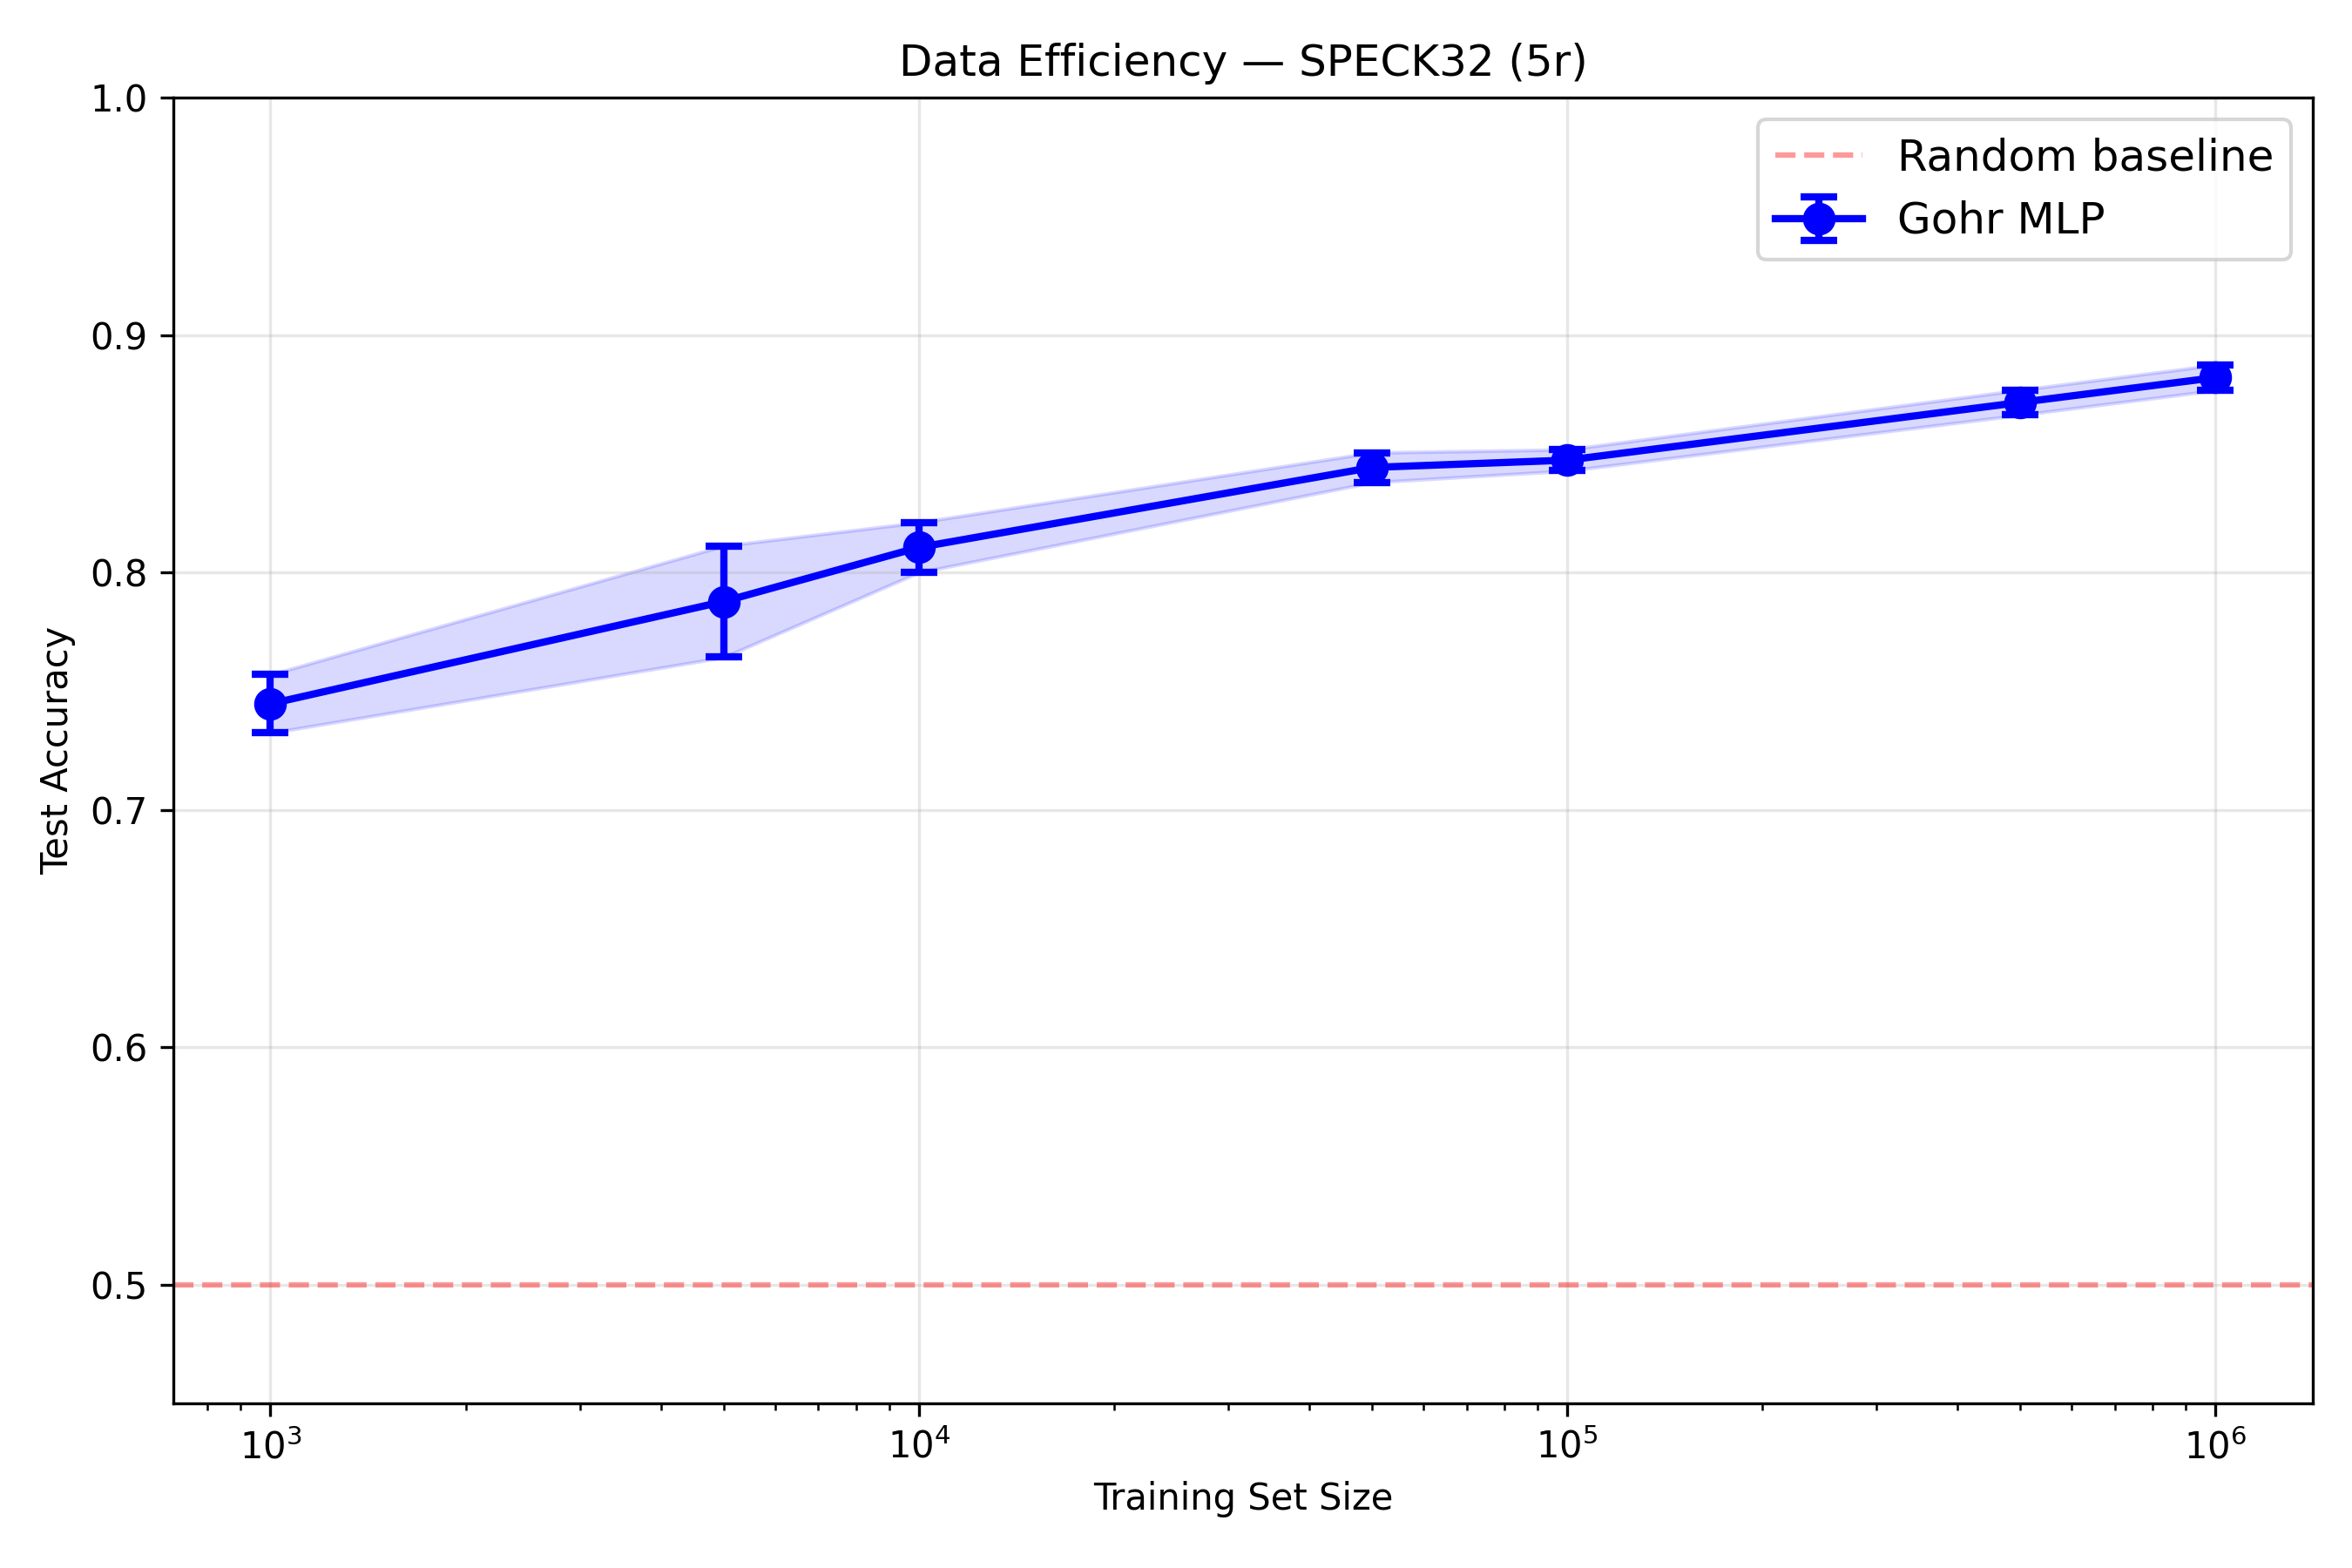
\includegraphics[width=0.85\textwidth]{e14_data_efficiency/e14_speck32_r5.png}

\textbf{1K samples $\Rightarrow$ 74.5\%}\\
(24.5pp above random)

Practical knee at $\sim$50--100K.\\
500K$\to$1M: only +1.1pp.
\end{column}
\end{columns}
\end{frame}

% ==============================================================================
% SLIDE 15: Transfer Learning
% ==============================================================================
\begin{frame}{No Cross-Round Transfer}
\small
\begin{columns}[c]
\begin{column}{0.54\textwidth}
\centering
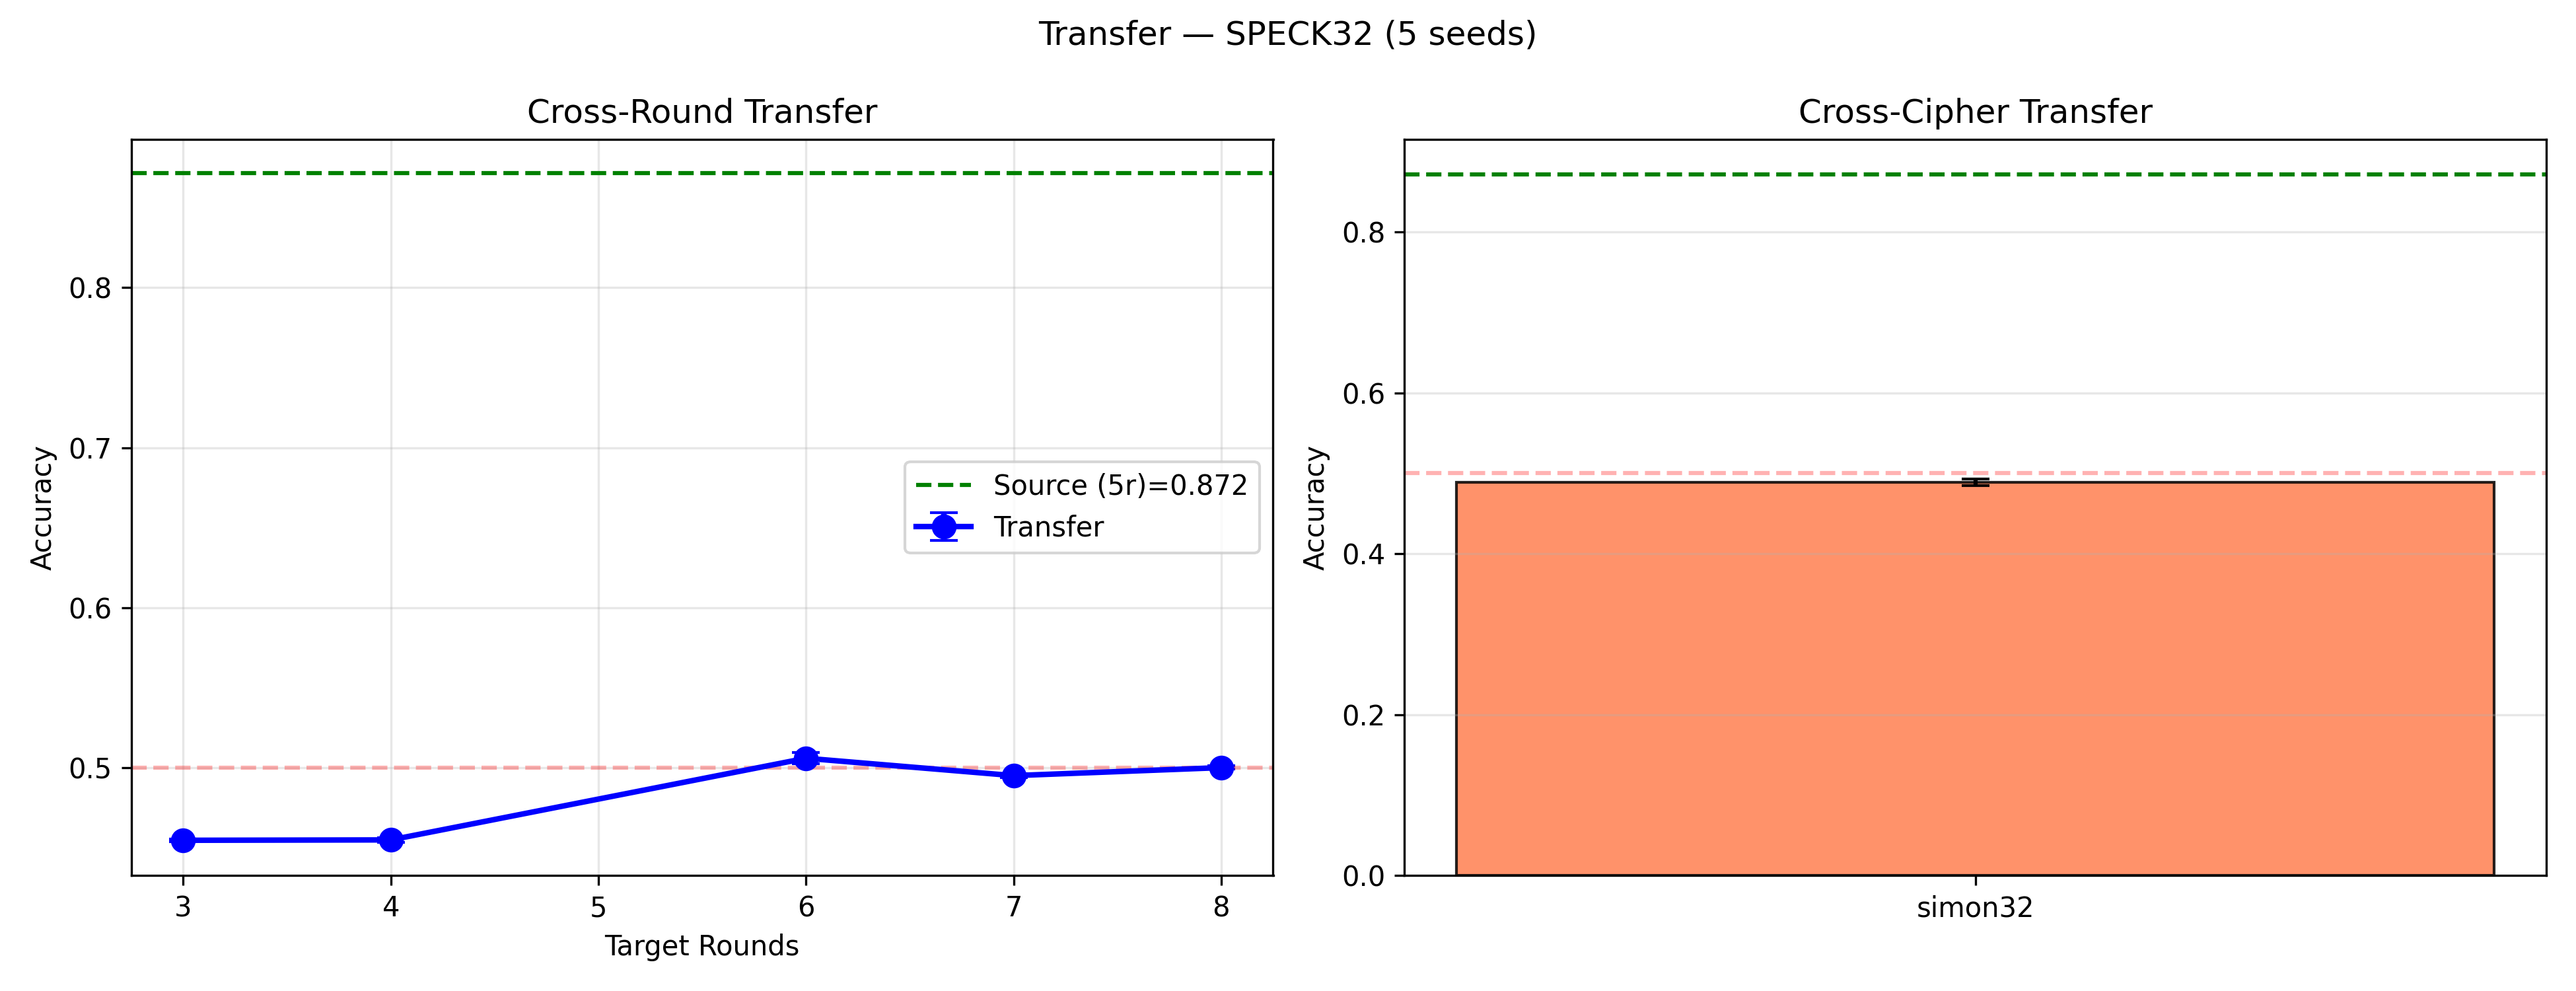
\includegraphics[width=0.9\textwidth]{e09_transfer/e09_speck32.png}
\end{column}
\begin{column}{0.43\textwidth}
5-round model, zero-shot on others:

\begin{tabular}{@{}cr@{}}
\toprule
\textbf{Target} & \textbf{Accuracy} \\
\midrule
3 rounds & 45.5\% \\
4 rounds & 45.5\% \\
\textit{5 (source)} & \textit{87.2\%} \\
6 rounds & 50.6\% \\
7 rounds & 49.5\% \\
\bottomrule
\end{tabular}

\textbf{Below 50\%} at 3--4 = \emph{worse than random}. The 5-round features are anti-correlated with 3--4 round structure.
\end{column}
\end{columns}
\end{frame}

% ==============================================================================
% SLIDE 16: Key Findings
% ==============================================================================
\begin{frame}{Key Findings}
\small
\begin{enumerate}
  \setlength{\itemsep}{0.2cm}
  \item[\checkmark] \textbf{Representation $>$ Architecture}\\
  Representation gap: 28.85pp vs.\ architecture gap: 3.89pp.\\
  XOR diff halves dimensionality with no accuracy loss.

  \item[\checkmark] \textbf{Markov Assumption Holds}\\
  Three independent validations: conditional MI $\approx 0$,
  generative ratio $\approx 1.0$, depth analysis consistent.

  \item[\checkmark] \textbf{Position-Specific Features Tied to Cipher Structure}\\
  37pp drop under permutation. Saliency identifies bits 14, 28, 12, 13, 29 --- matching SPECK's $\alpha\!=\!7$, $\beta\!=\!2$. Automated search confirms.
\end{enumerate}
\end{frame}

% ==============================================================================
% SLIDE 17: Contributions & Future Work
% ==============================================================================
\begin{frame}{Contributions \& Future Directions}
\small
\begin{columns}[T]
\begin{column}{0.48\textwidth}
\textbf{What we built:}
\begin{itemize}
  \item 15 experiments, 7 representations, 6 architectures
  \item 5-seed averaging + bootstrap CIs
  \item 46 unit tests, open-source PyTorch
  \item First systematic representation study for neural distinguishers
  \item Empirical Markov validation via 3 independent methods
\end{itemize}
\end{column}
\begin{column}{0.48\textwidth}
\textbf{What's next:}
\begin{itemize}
  \item Full Bayesian key-recovery attack
  \item Cross-cipher: SIMON32, PRESENT
  \item Close the 7-round gap (50.7\% vs.\ Gohr's 61.2\%)
  \item Neural round inversion for trail reconstruction
  \item Adversarial robustness beyond 5\% BER
\end{itemize}
\end{column}
\end{columns}

\vspace{0.2cm}
\centering
{\scriptsize \textbf{References:}
Gohr (CRYPTO '19) $\cdot$ Benamira et al.\ (EUROCRYPT '21) $\cdot$ Biham \& Shamir ('91) $\cdot$ Belghazi et al.\ (ICML '18) $\cdot$ Beaulieu et al.\ ('15)}
\end{frame}

% ==============================================================================
% SLIDE 18: Thank You
% ==============================================================================
\begin{frame}[plain]
  \begin{center}
    {\Huge Thank You!}

    \vspace{0.4cm}

    {\Large Questions?}

    \vspace{0.6cm}

    \textbf{Angadjeet Singh}\\[0.1cm]
    Roll Number: 2022071\\
    Applied Cryptography\\
    Department of CSE, IIIT Delhi

    \vspace{0.2cm}

    \texttt{angadjeet22071@iiitd.ac.in}

    \vspace{0.2cm}

    {\scriptsize \texttt{github.com/ANGADJEET/Neural-Cryptanalysis}}
  \end{center}
\end{frame}

% ==============================================================================
% BACKUP SLIDES
% ==============================================================================
\appendix



\end{document}
